%% abtex2-modelo-trabalho-academico.tex, v-1.9.6 laurocesar
%% Copyright 2012-2016 by abnTeX2 group at http://www.abntex.net.br/ 
%%
%% This work may be distributed and/or modified under the
%% conditions of the LaTeX Project Public License, either version 1.3
%% of this license or (at your option) any later version.
%% The latest version of this license is in
%%   http://www.latex-project.org/lppl.txt
%% and version 1.3 or later is part of all distributions of LaTeX
%% version 2005/12/01 or later.
%%
%% This work has the LPPL maintenance status `maintained'.
%% 
%% The Current Maintainer of this work is the abnTeX2 team, led
%% by Lauro César Araujo. Further information are available on 
%% http://www.abntex.net.br/
%%
%% This work consists of the files abntex2-modelo-trabalho-academico.tex,
%% abntex2-modelo-include-comandos and abntex2-modelo-references.bib
%%

% ------------------------------------------------------------------------
% ------------------------------------------------------------------------
% abnTeX2: Modelo de Trabalho Academico (tese de doutorado, dissertacao de
% mestrado e trabalhos monograficos em geral) em conformidade com 
% ABNT NBR 14724:2011: Informacao e documentacao - Trabalhos academicos -
% Apresentacao
% ------------------------------------------------------------------------
% ------------------------------------------------------------------------

\documentclass[
	% -- opções da classe memoir --
	12pt,				% tamanho da fonte
	openright,			% capítulos começam em pág ímpar (insere página vazia caso preciso)
	oneside,			% para impressão em recto e verso. Oposto a oneside
	a4paper,			% tamanho do papel. 
	% -- opções da classe abntex2 --
	%chapter=TITLE,		% títulos de capítulos convertidos em letras maiúsculas
	%section=TITLE,		% títulos de seções convertidos em letras maiúsculas
	%subsection=TITLE,	% títulos de subseções convertidos em letras maiúsculas
	%subsubsection=TITLE,% títulos de subsubseções convertidos em letras maiúsculas
	% -- opções do pacote babel --
	english,			% idioma adicional para hifenização
	%french,				% idioma adicional para hifenização
	%spanish,			% idioma adicional para hifenização
	brazil				% o último idioma é o principal do documento
	]{abntex2}

% ---
% Pacotes básicos 
% ---
\usepackage{lmodern}			% Usa a fonte Latin Modern			
\usepackage[T1]{fontenc}		% Selecao de codigos de fonte.
\usepackage[utf8]{inputenc}		% Codificacao do documento (conversão automática dos acentos)
\usepackage{lastpage}			% Usado pela Ficha catalográfica
\usepackage{indentfirst}		% Indenta o primeiro parágrafo de cada seção.
\usepackage{color}				% Controle das cores
\usepackage{graphicx}			% Inclusão de gráficos
\usepackage{microtype} 			% para melhorias de justificação
\usepackage{subfig}
\usepackage{float}
\usepackage{listofsymbols}

\usepackage{amsmath}
\usepackage{listings}
%\usepackage{xcolor}

%\usepackage{reledmac}


%pacote da tabela
\usepackage{multirow}
% ---
%	
% ---
% Pacotes adicionais, usados apenas no âmbito do Modelo Canônico do abnteX2
% ---
\usepackage{lipsum}				% para geração de dummy text
% ---

% ---
% Pacotes de citações
% ---
\usepackage[brazilian,hyperpageref]{backref}	 % Paginas com as citações na bibl
%\usepackage[alf]{abntex2cite}	% Citações padrão ABNT
\usepackage[alf,abnt-etal-list=0,abnt-etal-cite=3]{abntex2cite}
 
% --- 
% CONFIGURAÇÕES DE PACOTES
% --- 

% ---
% Configurações do pacote backref
% Usado sem a opção hyperpageref de backref
\renewcommand{\backrefpagesname}{Citado na(s) página(s):~}
% Texto padrão antes do número das páginas
\renewcommand{\backref}{}
% Define os textos da citação
\renewcommand*{\backrefalt}[4]{
	\ifcase #1 %
		Nenhuma citação no texto.%
	\or
		Citado na página #2.%
	\else
		Citado #1 vezes nas páginas #2.%
	\fi}%
% ---

% ---
% Informações de dados para CAPA e FOLHA DE ROSTO
% ---
\titulo{BioGlove: Protótipo de um transdutor de flexão bioinspirado}
\autor{Wederson Medeiros Silva}
\local{Belém -- Pará}
\data{2019}
\orientador{Prof. Dr. Roberto Menezes Rodrigues}
\coorientador{Prof. Dr. João Crisóstomo Weyl A. Costa}
\instituicao{
  Universidade Federal do Pará -- UFPa
  \par
  Instituto de Tecnologia -- ITEC
  \par
  Faculdade de Engenharia da Computação e Telecomunicações -- FCT}
\tipotrabalho{Trabalho de Conclusão de Curso}

% O preambulo deve conter o tipo do trabalho, o objetivo, 
% o nome da instituição e a área de concentração 
\preambulo{Trabalho de Conclusão de Curso apresentado para obtenção do
título de Bacharel em Engenharia da Computação. Instituto de Tecnologia. Faculdade de Engenharia da Computação e Telecomunicações. Universidade Federal do Pará.
}
% ---


% ---
% Configurações de aparência do PDF final

% alterando o aspecto da cor azul
\definecolor{blue}{RGB}{41,5,195}

% informações do PDF
\makeatletter
\hypersetup{
     	%pagebackref=true,
		pdftitle={\@title}, 
		pdfauthor={\@author},
    	pdfsubject={\imprimirpreambulo},
	    pdfcreator={LaTeX with abnTeX2},
		pdfkeywords={abnt}{latex}{abntex}{abntex2}{trabalho acadêmico}, 
		colorlinks=true,       		% false: boxed links; true: colored links
    	linkcolor=black,          	% color of internal links
    	citecolor=black,        		% color of links to bibliography
    	filecolor=black,      		% color of file links
		urlcolor=black,
		bookmarksdepth=4
}
\makeatother
% --- 

% --- 
% Espaçamentos entre linhas e parágrafos 
% --- 

% O tamanho do parágrafo é dado por:
\setlength{\parindent}{1.3cm}

% Controle do espaçamento entre um parágrafo e outro:
\setlength{\parskip}{0.2cm}  % tente também \onelineskip

% ---
% compila o indice
% ---
\makeindex
% ---

% ----
% Início do documento
% ----
\begin{document}

% Seleciona o idioma do documento (conforme pacotes do babel)
%\selectlanguage{english}
\selectlanguage{brazil}

% Retira espaço extra obsoleto entre as frases.
\frenchspacing 

% ----------------------------------------------------------
% ELEMENTOS PRÉ-TEXTUAIS
% ----------------------------------------------------------
% \pretextual

% ---
% Capa
% ---
\renewcommand{\imprimircapa}{
\begin{capa}

\center

\includegraphics[scale=0.4]{figures/ufpa_logo.jpg}

 { \ABNTEXchapterfont 
 UNIVERSIDADE FEDERAL DO PARÁ\\
 INSTITUTO DE TECNOLOGIA\\
 FACULDADE DE ENGENHARIA DA COMPUTAÇÃO E TELECOMUNICAÇÕES\\}
   \vspace*{4.0cm}
 
 { \ABNTEXchapterfont\large
   \textbf{\imprimirautor}}
   \vspace*{3.0cm}

 {\ABNTEXchapterfont\LARGE
 \textbf{\imprimirtitulo}}

 \vspace*{\fill}
 {\large\imprimirlocal}
 \par
 {\large\imprimirdata}
 \vspace*{1cm}
\end{capa}
}
% ---
% Capa
% ---
\imprimircapa
% ---

% ---
% Folha de rosto
% (o * indica que haverá a ficha bibliográfica)
% ---
%%Folha de Rosto
\makeatletter
\renewcommand{\folhaderostocontent}{
  \begin{center}

    \vspace*{0.08cm}
    {\ABNTEXchapterfont\Large
     \imprimirautor}

    \vspace*{\fill}\vspace*{\fill}
    {\ABNTEXchapterfont\LARGE
     \textbf{\imprimirtitulo}}
     \vspace*{\fill}

    \abntex@ifnotempty{\imprimirpreambulo}{
      \hspace{.45\textwidth}
      \begin{minipage}{.5\textwidth}
         \imprimirpreambulo\\    
      \end{minipage}%
       \vspace*{\fill}
    }%
    
    {\ABNTEXchapterfont\Large
     \imprimirorientadorRotulo
     \ABNTEXsectionfont~\imprimirorientador\par}
    
    {\ABNTEXchapterfont\Large
     \imprimircoorientadorRotulo
     \ABNTEXsectionfont~\imprimircoorientador}%

    \vspace*{\fill}
    {\large\imprimirlocal}
    \par
    {\large\imprimirdata}
  \end{center}
}
\makeatother

% ---
% Folha de rosto
% (o * indica que haverá a ficha bibliográfica)
% ---
\imprimirfolhaderosto*
% ---
% ---
% Inserir a ficha bibliografica
% ---

% Isto é um exemplo de Ficha Catalográfica, ou ``Dados internacionais de
% catalogação-na-publicação''. Você pode utilizar este modelo como referência. 
% Porém, provavelmente a biblioteca da sua universidade lhe fornecerá um PDF
% com a ficha catalográfica definitiva após a defesa do trabalho. Quando estiver
% com o documento, salve-o como PDF no diretório do seu projeto e substitua todo
% o conteúdo de implementação deste arquivo pelo comando abaixo:
%
% \begin{fichacatalografica}
%     \includepdf{fig_ficha_catalografica.pdf}
% \end{fichacatalografica}

\begin{fichacatalografica}
	\sffamily
	\vspace*{\fill}					% Posição vertical
	\begin{center}					% Minipage Centralizado
	\fbox{\begin{minipage}[c][8cm]{13.5cm}		% Largura
	\small
	\imprimirautor
	%Sobrenome, Nome do autor
	
	\hspace{0.5cm} \imprimirtitulo  / \imprimirautor. --
	\imprimirlocal, \imprimirdata-
	
	\hspace{0.5cm} \pageref{LastPage} p. : il. (algumas color.) ; 30 cm.\\
	
	\hspace{0.5cm} \imprimirorientadorRotulo~\imprimirorientador\\
	
	\hspace{0.5cm} \imprimircoorientadorRotulo~\imprimircoorientador\\
	
	\hspace{0.5cm}
	\parbox[t]{\textwidth}{\imprimirtipotrabalho~--~\imprimirinstituicao,
	\imprimirdata.}\\
	
	\hspace{0.5cm}
		1. Modo fantasma de segunda camada.
		2. Taxa agregada.
		3. \textit{Vectoring}.
		4. EVM.
		I. \imprimirorientador.
		II. Universidade Federal do Pará.
		III. Faculdade de Engenharia da Computação e Telecomunicações.
		IV. \imprimirtitulo\\ 		
	\end{minipage}}
	\end{center}
\end{fichacatalografica}
% ---
% ---

% ---
% Inserir folha de aprovação
% ---

% Isto é um exemplo de Folha de aprovação, elemento obrigatório da NBR
% 14724/2011 (seção 4.2.1.3). Você pode utilizar este modelo até a aprovação
% do trabalho. Após isso, substitua todo o conteúdo deste arquivo por uma
% imagem da página assinada pela banca com o comando abaixo:
%
% \includepdf{folhadeaprovacao_final.pdf}
%
\begin{folhadeaprovacao}

  \begin{center}
    {\ABNTEXchapterfont\large\imprimirautor}

    \vspace*{\fill}\vspace*{\fill}
    \begin{center}
      \ABNTEXchapterfont\bfseries\Large\imprimirtitulo
    \end{center}
    \vspace*{\fill}
    
    \hspace{.45\textwidth}
    \begin{minipage}{.5\textwidth}
        \imprimirpreambulo
    \end{minipage}%
    \vspace*{\fill}
   \end{center}
        
   Trabalho aprovado. \imprimirlocal, 18 de março de 2019:

   Conceito: .
   
   \assinatura{\textbf{\imprimirorientador} \\ Orientador} 
   \assinatura{\textbf{\imprimircoorientador} \\ Coorientador}
   \assinatura{\textbf{Prof. Dra. Josiane do Couto Rodrigues} \\ Convidado 1}
  % \assinatura{\textbf{Prof. Dr. Somebody else} \\ Convidado 2}
   %\assinatura{\textbf{Professor} \\ Convidado 3}
      
   \begin{center}
    \vspace*{0.5cm}
    {\large\imprimirlocal}
    \par
    {\large\imprimirdata}
    \vspace*{1cm}
  \end{center}
  
\end{folhadeaprovacao}
% ---

% ---
% Dedicatória
% ---
\begin{dedicatoria}
   \vspace*{\fill}
   \centering
   \noindent
   \textit{ Este trabalho é dedicado...} \vspace*{\fill}
\end{dedicatoria}
% ---

% ---
% Agradecimentos
% ---
\begin{agradecimentos}
Agradeço ao Professor Dr. ...
\end{agradecimentos}
% ---
% ---

% ---
% Epígrafe
% ---
\begin{epigrafe}
    \vspace*{\fill}
	\begin{flushright}
		\textit{``Talvez não tenha conseguido fazer o melhor, mas lutei para que o melhor fosse feito. \\ Não sou o que deveria ser, mas Graças a Deus, não sou o que era antes''. \\ (Martin Luther King)}
	\end{flushright}
\end{epigrafe}
% ---

% ---
% RESUMOS
% ---

% resumo em português
\setlength{\absparsep}{18pt} % ajusta o espaçamento dos parágrafos do resumo
\begin{resumo}
%\setlength{\parindent}{1.5cm}
%\indent
%\hangindent=3.7cm
	\hspace{1.5cm}Luvas embarcadas com sensores, também conhecidas como \textit{data gloves}, permitem diversas interações com realidade virtual, robótica, controle, internet das coisas, dentre outras. Dentro da luva, para que seja possível medir a flexão dos dedos, existem soluções baseadas em fibra óptica, tinta condutiva, potenciômetros e os mais conhecidos sensores flex. Entretanto, em muitos projetos, o custo da luva se torna elevado por conta da tecnologia escolhida para mensurar os graus de flexão em cada um dos dedos. Com o propósito de diminuir custos de projetos que necessitam de uma \textit{data glove}, foi desenvolvida a BioGlove, que é uma luva embarcada com sensores de flexão de baixo custo, placa microcontroladora que possui larga documentação e disponibilidade, além de um protocolo de comunicação simplificado. Além do mais, dentro do trabalho é proposto a avaliação de um sensor de flexão bioinspirado na mecânica dos dedos.


 \textbf{Palavras-chaves}: Data glove. BioGlove. sensor de flexão. bioinspirado. baixo custo.
\end{resumo}

% resumo em inglês
\begin{resumo}[Abstract]
 \begin{otherlanguage*}{english}
\hspace{1.5cm}Gloves embedded with sensors, also known as data gloves, allow various interactions with virtual reality, robotics, control, internet of things, and so on. Inside the glove, to be possible to measure finger flexion, there are solutions based on fiber optics, conductive ink, potentiometers and the well known flex sensors. However,
in many projects, the glove's cost become high because of technology chosen to measure fingers' degrees flexion. With the purpose of decrease costs of projects that need a data glove, was developed the BioGlove, that is a glove embedded with low cost flex sensors, microcontroller board with extensive documentation and availability, as well as a simplified communication protocol. Furthermore, in the work is proposed the avaliation of a flex sensor bioinspired by finger mechanics.



   \vspace{\onelineskip}
 
   \noindent 
   \textbf{Keywords}: Data glove. BioGlove. flex sensor. bioinspired. low cost.
 \end{otherlanguage*}
\end{resumo}


% ---
% inserir lista de ilustrações
% ---
\pdfbookmark[0]{\listfigurename}{lof}
\listoffigures*
\cleardoublepage
% ---

% ---
% inserir lista de tabelas
% ---
\pdfbookmark[0]{\listtablename}{lot}
\listoftables*
\cleardoublepage
% ---

% ---
% inserir lista de abreviaturas e siglas
% ---
%\imprimirlistadesiglas
\begin{siglas}

	\item[AM]\textit{Amplitude Modulation}
	\item[I]Corrente elétrica
	\item[IDE]\textit{Integrated Development Interface}
	\item[$k\Omega$]\textit{Quiloohm}
	\item[LED]\textit{Light-Emitting Diode}
	\item[LiPo]\textit{Lithium-ion Polymer}
	\item[$mAh$]Miliampere hora
	\item[$MHz$]Megahertz
	\item[mm]Milímetro
	\item[PCI]Placa de Circuito Impresso
	\item[PVC]\textit{Polyvinyl Chloride}	
	\item[R]Resistência elétrica
	\item[RF]Radio frequência
	\item[V]Tensão

		% --- Parte baseado em: http://www.inmetro.gov.br/consumidor/pdf/Resumo_SI.pdf
	
\end{siglas}
% ---

% ---
% inserir lista de símbolos
% ---


%\begin{simbolos}
%  \item[$\alpha$] Contante de atenuação
%  \item[$\beta$] Contante de fase
%  \item[$\gamma$] Contante de propagação
%  \item[$\Gamma_{L}$] Coeficiente de reflexão na carga
%  \item[$\delta$] Constante da restrição de potência transmissão
%  \item[$\Delta_f$ ] Subcanais ou tons em Hz
%  \item[$ \Gamma $]  Gap de $RSIR$
%  \item[$ \Lambda $] Matriz que contém os elementos da diagonal principal de $\mathbf{H}$
%  \item[$\rho$] Máscara espectral utilizada pelo sistema DSL
  %  \item[
%  \item[${\sigma}^{2}$]  Densidade espectral de potência potência do ruído Gaussiano branco aditivo
%\end{simbolos}


% ---

% ---
% inserir o sumario
% ---
\pdfbookmark[0]{\contentsname}{toc}
\tableofcontents*
\cleardoublepage
% ---



% ----------------------------------------------------------
% GUIA DAYNARA
% ----------------------------------------------------------
%{\color{green}
%1- Introdução 
%
%Seção 1: Contexto:
%
%	-Contexto da tecnologia, contendo um histórico das evoluções ADSL – VDSL – G. Fast 
%	
%	-Apontar limitações dos sistemas em relação a transmissão (taxa agregada)
%	
%	-Quais as soluções que estão sendo investigadas
%	
%	-Uma das soluções é buscar modos de transmissão alternativos
%	
%	-Modo fantasma, split-pair e wire-shield 
%	
%Seção 2: Trabalhos relacionados (até onde eles abordaram)
%
%Seção 3: *Motivação:
%Por que pesquisar esta área e esse tema de modos alternativos de transmissão, onde poderia ser aplicados (5G, XG.), etc.;
%
%Seção 4: *Justificativa:
%Quais são exatamente as contribuições, o que eu fiz a mais em relação ao que já existe.
%
%Seção 6:*Objetivos
%
%Seção 5:*Resumo da metodologia
%
%Seção :*organização do trabalho
%}
%{\color{red}


% ----------------------------------------------------------
% ELEMENTOS TEXTUAIS
% ----------------------------------------------------------
\textual

\chapter{Introdução} % ou \input{arquivoexterno}
		
		\section{Contextualização}

%		A biologia inspira diversos projetos de engenharia. Na área da robótica, por exemplo, existe um robô em formato de salamandra que é capaz de se movimentar bem entre a água e a terra, há um pequeno robô inspirado em moscas que, devido ao seu formato, possui excelente decolagem vertical na hora do vôo. Existe ainda um robô que consegue escalar paredes através de um material adesivo que foi inspirado pela lagartixa \cite{pfeifer2007biorobot}. 

		A biologia intriga e inspira a humanidade desde a antiguidade, a diversidade dos seres vivos observáveis em suas mais diversas formas e capacidades geram questionamentos e pesquisas até os dias de hoje. 

		Ainda na Grécia antiga, os pássaros com a sua capacidade natural de voar, serviram de base para um dos primeiros projetos bioinspirados de que se tem notícia. Acredita-se que por volta de 400 a.C., Archytas (430 - 360 a.C.) que foi um matemático e astrônomo, inventou uma pomba mecânica que deveria voar \cite{livingstone2014greece}. Leonardo Da Vinci (1452 - 1519 d.C.), provavelmente inspirado pelo projeto de Archytas, criou uma pomba mecânica que deslizava sobre um cabo ao mesmo tempo em que batia suas asas. Tempos depois, por volta do século XIX, um dispositivo muito parecido era vendido como brinquedo \cite{rosheim2006leonardo}.

		Atualmente, dentre os materiais bioinspirados mais famosos está a tecnologia VELCRO${\textregistered}$ que foi baseada em uma planta chamada Bardana (\textit{Arctium lappa}). Essa planta possui uma série de pequenos ganchos que grudam em alguns tecidos. Por conta desse comportamento, o VELCRO${\textregistered}$ é composto de duas partes, os ganchos e as voltas \cite{velcro2019about}. Especificamente na área da robótica, existe um robô em formato de salamandra que é capaz de se movimentar bem entre a água e a terra, há um pequeno robô inspirado na mosca que, devido ao seu formato, possui excelente decolagem vertical na hora do vôo. Existe ainda um robô que consegue escalar paredes através de um material adesivo que foi inspirado pela lagartixa \cite{pfeifer2007biorobot}. 

		Contudo, ao longo dos anos, não somente os animais e plantas vem servindo de base para projetos de engenharia. O próprio Leonardo da Vinci, por exemplo, a partir dos seus estudos em corpos humanos dissecados, chegou a construir modelos mecânicos de músculos, juntas, braços, entre outros que foram usados em muitas de suas invenções \cite{rosheim2006leonardo}.
		
		Especificamente sobre a mão, sabemos que ela exerce uma importante função na interação do ser humano com diversas ferramentas do dia a dia, desde o uso de instrumentos de trabalho como o martelo, serrote e a chave de fenda, até o ato de manipular a comida usando garfo e faca para se alimentar. Na área da tecnologia, muitos periféricos também necessitam da mão para serem controlados, é o caso do teclado do computador, do controle remoto da televisão e dos famosos tablets e smartphones.	Entretando, em aplicações de realidade virtual a imersão se torna ainda melhor quando são usados movimentos naturais do ser humano. Em um jogo de realidade virtual, por exemplo, será muito mais natural para o jogador alcançar um objeto virtual extendendo a sua mão, do que usar um \textit{joystick} para isso. Neste caso especificamente, o uso de uma luva embarcada com diversos sensores pode deixar a interação ainda mais real para o usuário. 
	

		\section{Estado da arte}

		
		Luvas embarcadas com sensores podem captar diversos movimentos das mãos, flexão dos dedos, giro do pulso, ou até mesmo saber a altura da mão em relação ao solo. Com isso é possível realizar o controle de outros equipamentos, estudar movimentos individuais de cada usuário afim de detectar limitações, desenvolver dispositivos que auxiliem em tratamentos dessa região, além de ser capaz de receber e transmitir diversas informações relevantes a cada caso.

		Dentre os trabalhos que envolvem luvas sensorizadas, existe um estudo de mapeamento dos movimentos do braço para controle de um braço robótico, onde os movimentos de flexão e extensão de um dos dedos e do pulso são adquiridos através de dois sensores resistivos de flexão comerciais, e um acelerômetro é responsável por mensurar movimentos do cotovelo. Esses dados são processados por um microcontrolador que por sua vez controla 4 servo motores montados em uma estrutura semelhante à de um braço robótico. Tal estrutura busca copiar os movimentos do braço do usuário através de 3 movimentos, ou graus de liberdade, independentes \cite{syed2012armcontroller}. Neste estudo é possível verificar que há uma conversão dos sinais analógicos em sinais digitais de uma forma proporcional, porém limitada. Além disso, o autor sugere que futuramente sejam adicionados protocolos para transmissão sem fio do sinal, o que pode dar uma maior liberdade de aplicações.
		
		Para auxiliar na área médica, por exemplo, foi desenvolvido o estudo de uma luva adaptável para medir a flexão dos dedos de indivíduos com limitações nos movimentos da mão e dos dedos \cite{simone2004lowcost}. O trabalho visa ser de baixo custo, limitar minimamente os movimentos naturais dos usuários, ser leve e de fácil aplicação e remoção. Tais requisitos servem para monitorar da melhor forma possível as atividades de pessoas com limitações de movimento em suas atividades diárias. Essa pesquisa também utiliza sensores resistivos de flexão comerciais nos cinco dedos da mão colados através de diferentes materiais. Usando uma espécie de caixa de conexões, um computador é ligado à todos os sensores e realiza a conversão dos sinais analógicos em sinais digitais. Os dados são salvos à uma frequência de 100 vezes por segundo usando o software proprietário LabView. Os testes mostraram que apesar de os sensores responderem aos movimentos, ainda é preciso realizar uma calibração antes do uso, além de que alguns materiais adesivos que grudavam os sensores aos dedos, acabaram soltando após algum período de uso. Por ser uma aplicação que visa ser utilizada durante testes relativamente longos (cerca de 24 horas), a necessidade de ter um computador conectado constantemente aos sensores pode de certa forma atrapalhar nas atividades de cada usuário durante os testes. Talvez o uso de um computador menor, Raspberry Pi por exemplo, poderia melhorar esse aspecto durante os testes.

		A 5DT Data Glove Ultra é uma espécie de luva sensorizada comercial que consegue capturar diversos movimentos da mão. Seus sensores de flexão são baseados em fibra ótica, possui opção para transmissão de dados sem fio através de Bluetooth, além de poder ser integrado à softwares de movimento e animação em 3D conhecidos no mercado. Também possui seu próprio software de diagnóstico, gerenciamento, calibração e gravação de dados \cite{5DT-ultra}. Todas essas características, fazem deste produto uma excelente ferramenta para realizar estudos sobre os movimentos das mãos, ou para o desenvolvimento e controle de outros produtos. Entretanto, seu custo pode chegar na faixa dos 1000 Dólares \cite{5DT-glove2019ebay}, o que pode ser um custo elevado para alguns usuários ou pesquisadores, além do mais, adaptações do hardware ou software que se fizerem necessárias, provavelmente não serão permitidas pelos desenvolvedores que detém os direitos deste produto.



%movimentar desenhos tridimencionais em computador \cite{5DT-ultra}, mensurar atividades de pessoas com limitações dos movimentos nos dedos \cite{simone2004lowcost} e até mesmo transcrever gestos em palavras baseado na linguagem americana de sinais \cite{anbarasi2013deafmute}. Existem produtos comerciais \cite{5DT-ultra}, projetos de baixo custo \cite{simone2004lowcost}, usados em pesquisas médicas \cite{michela2013rehab}, entre outros. 


%		Para flexionar os dedos das mãos, possuímos tendões que passam por dentro de polias. Quando o músculo atrelado à esses tendões de movimenta, obtém-se a flexão ou extensão dos dedos \cite{drricardocirurgiao}.

		
%		As funções atribuídas à essas luvas são variadas.		
		
		
		\section{Motivação}

		Apesar da gama de possibilidades com o uso de luvas sensorizadas, seu custo de montagem ou a obtenção de produtos comerciais possui custo elevado. Muitos projetos utilizam pelo menos 1 sensor flex em cada dedo, a compra de cada unidade desse sensor pode custar em lojas online especializadas em torno de 130 Reais \cite{multilogicaflexsensor}. Além disso, produtos comerciais costumam ter um hardware imutável e de difícil manutenção, pois somente equipes especializadas possuem o conhecimento técnico para efetuar reparos.

		O trabalho proposto busca criar um protótipo de uma luva embarcada com sensor de flexão, microcontrolador e transmissor de dados. O sistema deve possuir um conjunto de software e hardware que seja mais flexível em relação à outros produtos, permitindo que o usuário tenha liberdade de realizar modificações que se adaptem às suas necessidades. 

		Um dos componentes em maior número e de maior custo em projetos de luvas como essa, são os sensores de flexão. Portanto esse trabalho também propõe avaliar a viabilidade de um sistema transdutor de flexão inspirado no movimento dos músculos e tendões da mão. Esse sensor deverá ser composto de materiais de baixo custo e de fácil acesso.

		
		\section{Organização do trabalho}

		Este trabalho está organizado da seguinte forma:

		No capítulo 2 apresenta-se a mecânica que inspirou a construção do sensor, o funcionamento da aquisição dos movimentos, detalhes sobre o potenciômetro que é a peça chave do sensor, e por fim, as características do microcontrolador e transmissor utilizados.
		
		No capítulo 3 expõe-se mais detalhadamente o funcionamento do sensor, a adaptação do sensor na luva, o algoritmo de programação do software que trata o sinal recebido, os ajustes que foram necessários, além do protocolo de comunicação criado. Ao final é explicitado como todo o sistema foi construído e montado.

		No capítulo 4 os resultados e análises dos testes realizados na BioGlove, em comparação à outras luvas desenvolvidas, são mostrados.

		Por fim, no capítulo 5 são apresentas as conclusão do trabalho.
		

%Contextualização; Estado da arte (se tiver); Motivação; O que vai fazer; Metodologia; O que terá no resto do documento;




	% --------------------- 
	%	REFERENCIAL TEÓRICO	
	% --------------------- 
	
	\chapter{Referencial Teórico}

		\section{Introdução}

		Ao longo dos últimos anos, diversos trabalhos estão sendo realizados para mensurar os movimentos da mão e estes possuem as mais variadas motivações. A pesquisa de \cite{daeholee2009vision}, por exemplo, criou um controle remoto baseado na abertura dos dedos. O sistema processa imagens de uma câmera em busca de comandos pré-configurados que respondem a abertura de dedos da mão. Ou seja, mostrou-se a possibilidade de usar os movimentos da mão como um meio para controle remoto. Além disso, existem trabalhos como \cite{solanki2013sign} e \cite{anbarasi2013deafmute} que buscam traduzir gestos das mãos em palavras, buscando assim facilitar a comunicação de surdos e/ou mudos com outras pessoas. Já \cite{kumar2012hci} buscam uma interação humano-computador através do uso de uma luva. Nesse trabalho o autor demonstra que é possível realizar ações no computador, como desenhar ou manipular objetos tridimencionais, através de movimentos da mão pré-determinados.

		Dentre os produtos que ficaram famosos usando o movimentos das mãos para controle, estão as luvas \textit{Data Glove} e a \textit{Power Glove}, ambas criadas nos anos 80. A primeira, foi desenvolvida por volta de 1986 e era usada para controlar um supercomputador, mas também foi utilizada pela \textit{NASA (National Aeronautics and Space Administration)} para controlar robôs. Logo depois, por volta de 1987, uma licença foi comprada para desenvolver uma outra versão da luva, só que seria para uso do público em geral. Então, finalmente em 1989, através de uma parceria entre as empresas Mattel, Nintendo e AGE, foi lançada a \textit{Power Glove} que serviria para controlar jogos de videogames \cite{dana1989powerglove}.

		Entre os demais sistemas que buscam mensurar flexão e extensão dos dedos estão \cite{syed2012armcontroller} e \cite{michela2013rehab}. Estes e outros trabalhos, incluindo o trabalho proposto, nos quais utilizam luvas para auxiliar a captura dos movimentos dos dedos, costumam ter um bloco de funcionamento parecido ao da figura \ref{Fig:flowchart1}.


		\begin{figure}[h!]
			\centering
			\caption{Funcionamento de sistemas baseados em luvas}
  		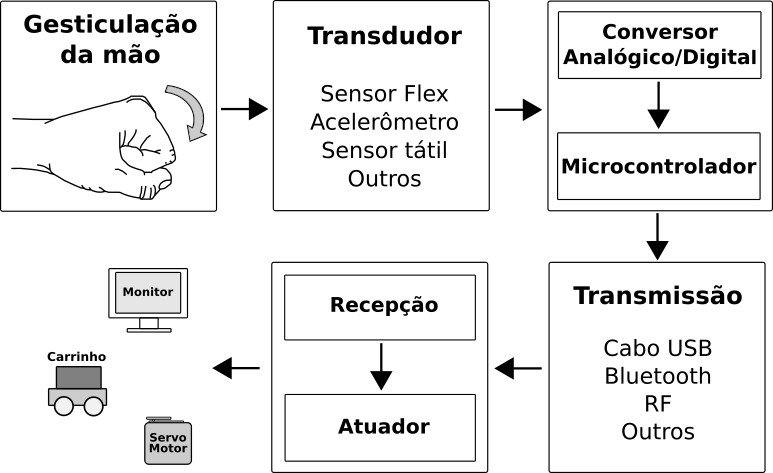
\includegraphics[width=10cm]{./figures/flowchart1.png}
  		\label{Fig:flowchart1}
			\fonte{Produzido pelo autor.}
		\end{figure}


		\section{Movimentação dos dedos} \label{movimentacaodosdedos}


		Na mão, os tendões funcionam como cordas que conectam os músculos do antebraço aos ossos da mão. Nos dedos, os tendões passam por dentro de uma série de polias, que formam uma espécie de túnel. Isso permite manter os tendões próximos aos ossos da mão, aumentando a força nos dedos e diminuindo o gasto de energia. Ao movimentar o dedo, o músculo se contrai para que o tendão deslize por entre as polias \cite{drricardocirurgiao}. Semelhante ao esquema demonstrado na figura \ref{Fig:hand-tendon-flex1-and-exo-glove1} (a).



	\begin{figure}[!htb]
		 \centering
		 \caption{(a) Movimento através do tendão e (b) \textit{Exo-Glove} instalada.} 
		 \subfloat[]
		 {
			 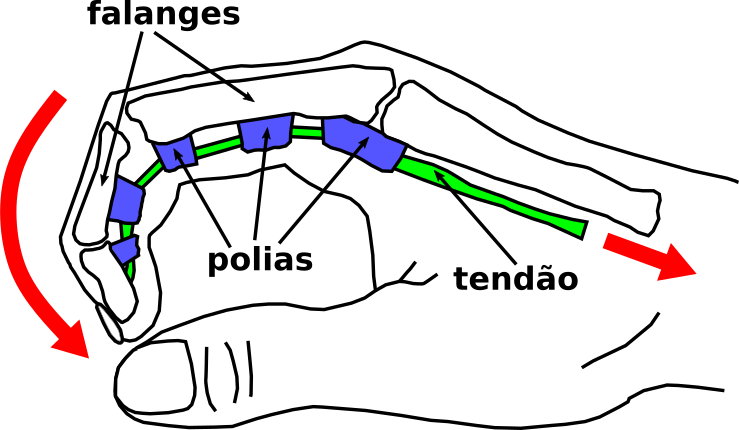
\includegraphics[width=8cm,keepaspectratio=true]{./figures/hand-tendon-flex1.png}
		 }
		 \centering
		 \subfloat[]
		 { 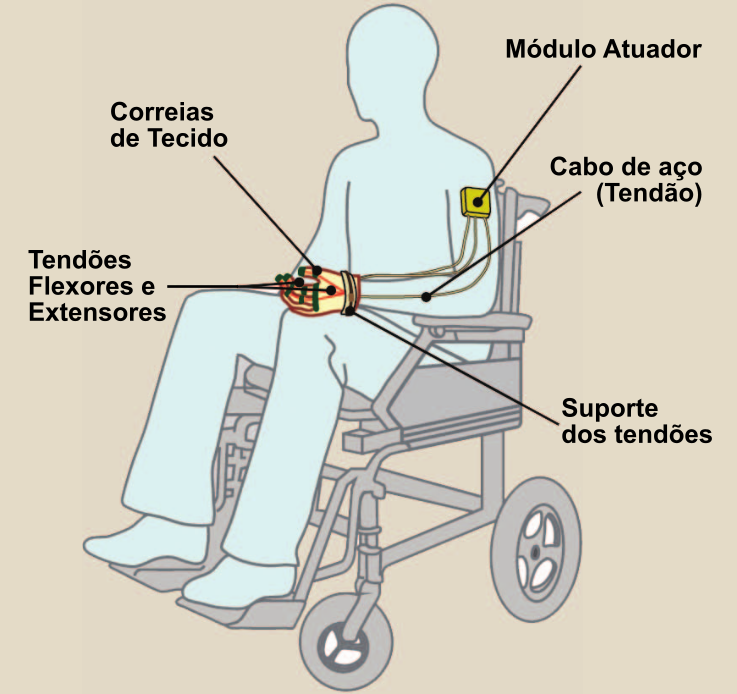
\includegraphics[width=6cm,keepaspectratio=true]{./figures/exo-glove-installed1.png}
		 }
		 \label{Fig:hand-tendon-flex1-and-exo-glove1}
		 \fonte{(a) Adaptado de \cite{drmarksurgery} e (b) adaptado de \cite{hyunki2015exoglove}.}
	\end{figure}

%		\begin{figure}[h!]
%			\centering
%  		\caption{Movimento do dedo através do tendão.}
%  		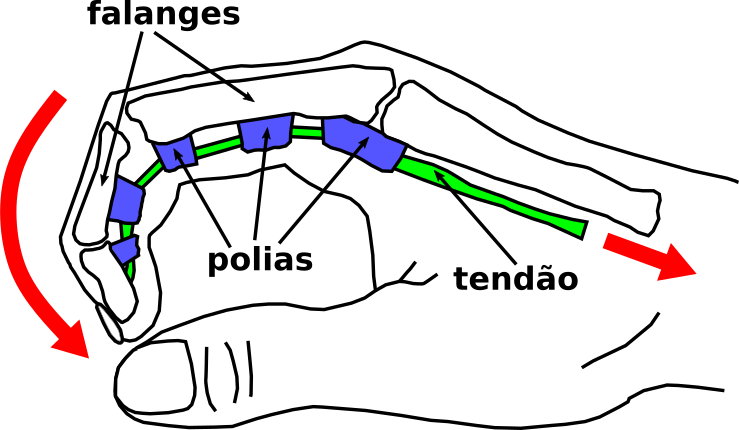
\includegraphics[scale=0.5]{./figures/hand-tendon-flex1.png}
%			\fonte{Adaptado de \cite{drmarksurgery}.}
%  		\label{Fig:hand-tendon-flex1}
%		\end{figure}

		Existem pesquisas inspiradas nessa biomecânica. Em \cite{hyunki2015exoglove}, por exemplo, mostra-se o funcionamento  da \textit{Exo-Glove}, que é uma luva que auxilia o movimento dos dedos da mão de pessoas que sofreram alguma paralisia na região. O sistema rotea tendões artificiais (cabos de aço) vindos de um módulo atuador, passando por um suporte próximo ao pulso, por correias de tecido e chegando até os dedos. Usando esse aparato, os movimentos de flexão e extensão dos dedos são auxiliados pelos cabos, tornando estes movimentos mais firmes ao usuário. A figura \ref{Fig:hand-tendon-flex1-and-exo-glove1} (b) demonstra o sistema descrito.

%		\begin{figure}[h!]
%			\centering
%			\caption{\textit{Exo-Glove} instalada em um cadeirante}
%  		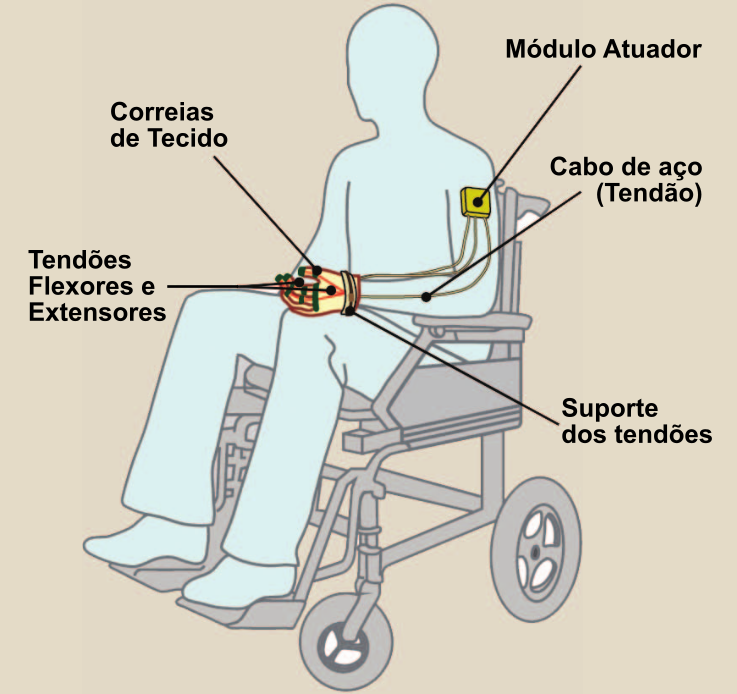
\includegraphics[scale=0.5]{./figures/exo-glove-installed1.png}
%			\fonte{Adaptado de \cite{hyunki2015exoglove}.}
%  		\label{Fig:exo-glove-installed1}
%		\end{figure}
		
		\section{Captura de movimentos}



		Os circuitos eletrônicos trabalham com sinais elétricos, ou seja, com correntes e tensões elétricas. Sendo assim, para medir grandezas físicas que não envolvam eletricidade, é preciso o uso de transdutores, que são dispositivos que convertem uma forma de energia em outra. Os transdutores muitas vezes são usados para sensoriar determinadas grandezas, e por conta disso também são conhecidos como sensores \cite{ncb2012eletronicabasica}.

		Muitas pesquisas que buscam mensurar os movimentos de flexão e expansão dos dedos, usam sensores de flexão comerciais semelhantes a \cite{flexsensor}. O trabalho de \cite{anbarasi2013deafmute} traduz gestos definidos na linguagem americana de sinais em texto e áudio. Dessa forma, há uma melhor comunicação de pessoas surdas ou mudas com outras pessoas que não são familiarizadas com a linguagem de sinais. A captura de flexões e extensões dos dedos são realizadas por sensores de flexão, enquanto que as direções, durante os gestos da mão, são captados por um acelerômetro. Um microcontrolador reconhece os movimentos, gera palavras e as converte em aúdio através de um módulo. 

		A \textit{Data Glove} usava fibra óptica e fotoresistores para saber as posições de cada dedo. De acordo com a flexão do sensor, o nível de luz que chegava ao fotoresistor variava indicando a posição atual. Já a \textit{Power Glove}, buscou reduzir custos e preferiu trocar essa tecnologia. Passou a usar placas com tintas que variavam suas propriedades condutivas quando torcidas \cite{dana1989powerglove}.

%		Neste trabalho, propo\~e-se criar um sistema inspirado na biomecâmica dos dedos. Esse sistema deve mensurar movimentos de flexão e extensão dos dedos usando um transdutor mecânico com funcionamento semelhante ao sistema de tendões que ocorre nas mãos. 




		\section{Potenciômetro}
		O potenciômetro é um componente eletrônico que permite, através do giro do seu eixo, a variação da resistência entre seus terminais. Eles são constituídos por um elemento de resistência, que pode ser de carbono ou fio de nicromo, sobre o qual corre uma lingueta, denominada cursor. Dentre as características do potenciômetro estão o valor máximo de sua resistência, seu número de voltas, seu grau máximo de giro (aproximado) e se ele é do tipo linear ou logarítmico \cite{ncb2012eletronicabasica}.


		\begin{figure}[h!]
			\centering
  		\caption{Funcionamento do potenciômetro linear.}
  		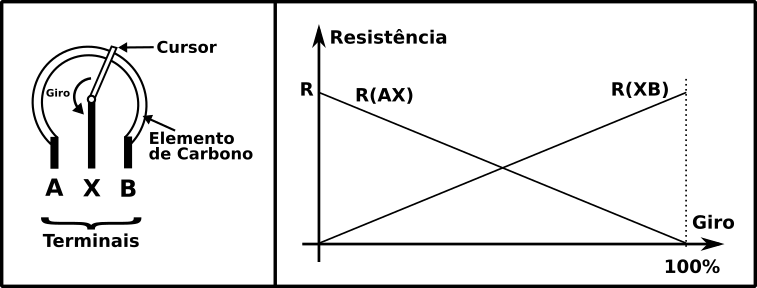
\includegraphics[width=12cm]{./figures/potentiometer1.png}
			\fonte{Modificado de~\cite{ncb2012eletronicabasica}.}
  		\label{Fig:potentiometer1}
		\end{figure}

		A figura \ref{Fig:potentiometer1} demonstra resumidamente o funcionamento do potenciômetro linear, a saída dos terminais é variada de acordo com o giro do cursor. Segundo a lei de Ohm ($V = R.I$), dada uma corrente constante, ao variar a resistência teremos uma variação da tensão. Sendo assim, ao girar o eixo do potenciômetro, dependendo do sentido do giro, perceberemos um aumento ou diminuição da tensão naquele ponto. Partindo de um ponto extremo com resistência mínima até o outro no qual a resistência deverá ser a máxima característica do componente.


		\section{Microcontroladores}

		Por volta da década de 80 surgiram os primeiros microcontroladores, dispositivos com memória RAM (\textit{Ramdon Access Memory}), ROM (\textit{Read Only Memory}), clock interno, E/S (Entrada e Saída), entre outros. Por conta dessas características, os microcontroladores permitiram que projetos de dispositivos inteligentes se tornassem mais simples. Eles eram chamados por muitas vezes de computadores em um único chip \cite{pereiramicrocontroladores}. 

		Em \cite{michela2013rehab} o microcontrolador HC9S08QB8, da fabricante Freescale, consegue trabalhar na faixa de tensão requerida pelo projeto, consume pouca energia e juntamente ao transceptor MAX 1412 é capaz de diminuir a complexidade de transmissão, além de outras características. Já em \cite{anbarasi2013deafmute}, o microcontrolador ATmega 328 é utilizado para mostrar uma saída de texto em uma pequena tela LCD e juntamente ao chip TTS256 converter esse texto em som.

		Existem ainda, soluções que buscam facilitar o uso do microcontrolador. o Arduino é uma plataforma eletrônica de código aberto que é baseada em \textit{hardware} e \textit{software} fáceis de usar. As placas Arduino são capazes de ler entradas como o acionamento de um sensor ou pressionamento de um botão. Pode transformar essas entradas em saídas como a ativação de um motor ou a publicação de algo online. Essa placa pode ser programada usando sua IDE (\textit{Integrated Development Interface}), que por sua vez, envia as instruções necessárias para o microcontrolador instalado na placa.\cite{arduinosite} 

		No trabalho proposto, a placa Arduino modelo Nano com o microcontrolador ATmega328 embarcado, é utilizada para receber os sinais dos transdutores, converter os sinais analógicos em digitais, codificar estes sinais e enviá-los. A figura \ref{Fig:arduino-nano1} mostra a placa utilizada no projeto.
		
		\begin{figure}[h!]
			\centering
			\caption{Placa Arduino modelo Nano.}
  		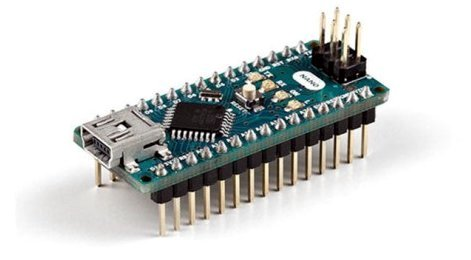
\includegraphics[width=12cm]{./figures/arduino-nano1.jpg}
  		\label{Fig:arduino-nano1}
			\fonte{Produzido pelo autor.}
		\end{figure}


		\section{Transmissão de Sinal}
		
		Existem várias formas de transmissão de sinal em projetos com luvas. Em \cite{solanki2013sign}, através de fios, a saída de texto do microcontrolador é transmitida e mostrada em uma pequena tela de LCD. No trabalho de \cite{syed2012armcontroller} os fios conectam o microcontrolador diretamente à servomotores que controlam um braço robótico.

		Para transmissões sem fio existem diversas opções. Na Power Glove \cite{dana1989powerglove} o sistema utilizado foi o ultrassom. Sendo que, na luva dois emissores de som ultrassonico enviam as informações necessárias para dois microfones localizados próximos à TV. Já o trabalho de \cite{kumar2012hci} utiliza a DG5 VHand 2.0 em sua pesquisa. Essa é uma luva comercial equipada com sensores detectores de flexão e movimentos, que usa Bluetooth para se comunicar com o computador.
		
		Em \cite{michela2013rehab}, a transmissão de sinal é realizada via rádio frequência, com o auxílio de um transceptor. Um transceptor é um sistema no qual estão presentes tanto o transmissor quanto o receptor de sinal em um mesmo módulo \cite{scott2017transceiver}.

		Outra opção para usar transmissão em rádio frequência é usar o receptor e o transmissor separadamente. No trabalho proposto usa-se o módulo RF (Rádio Frequência) 433 MHz, composto por um par que contém um transmissor (modelo XY-FST) e um receptor (modelo XY-MK-5V), ambos mostrados na figura \ref{Fig:tx-rx1}. O par opera com modulação AM (\textit{Amplitude Modulation}) e é considerado uma alternativa para projetos de baixo custo que queiram usar comunicação sem fio entre microcontroladores Arduino ou entre outros. O par de módulos pode alcançar até 200 metros sem obstáculos, usando antenas e dependendo da tensão aplicada \cite{institutodigitalrf}.


		\begin{figure}[h!]
			\centering
			\caption{Módulos RF transmissor (esq.) e receptor (dir.).}
  		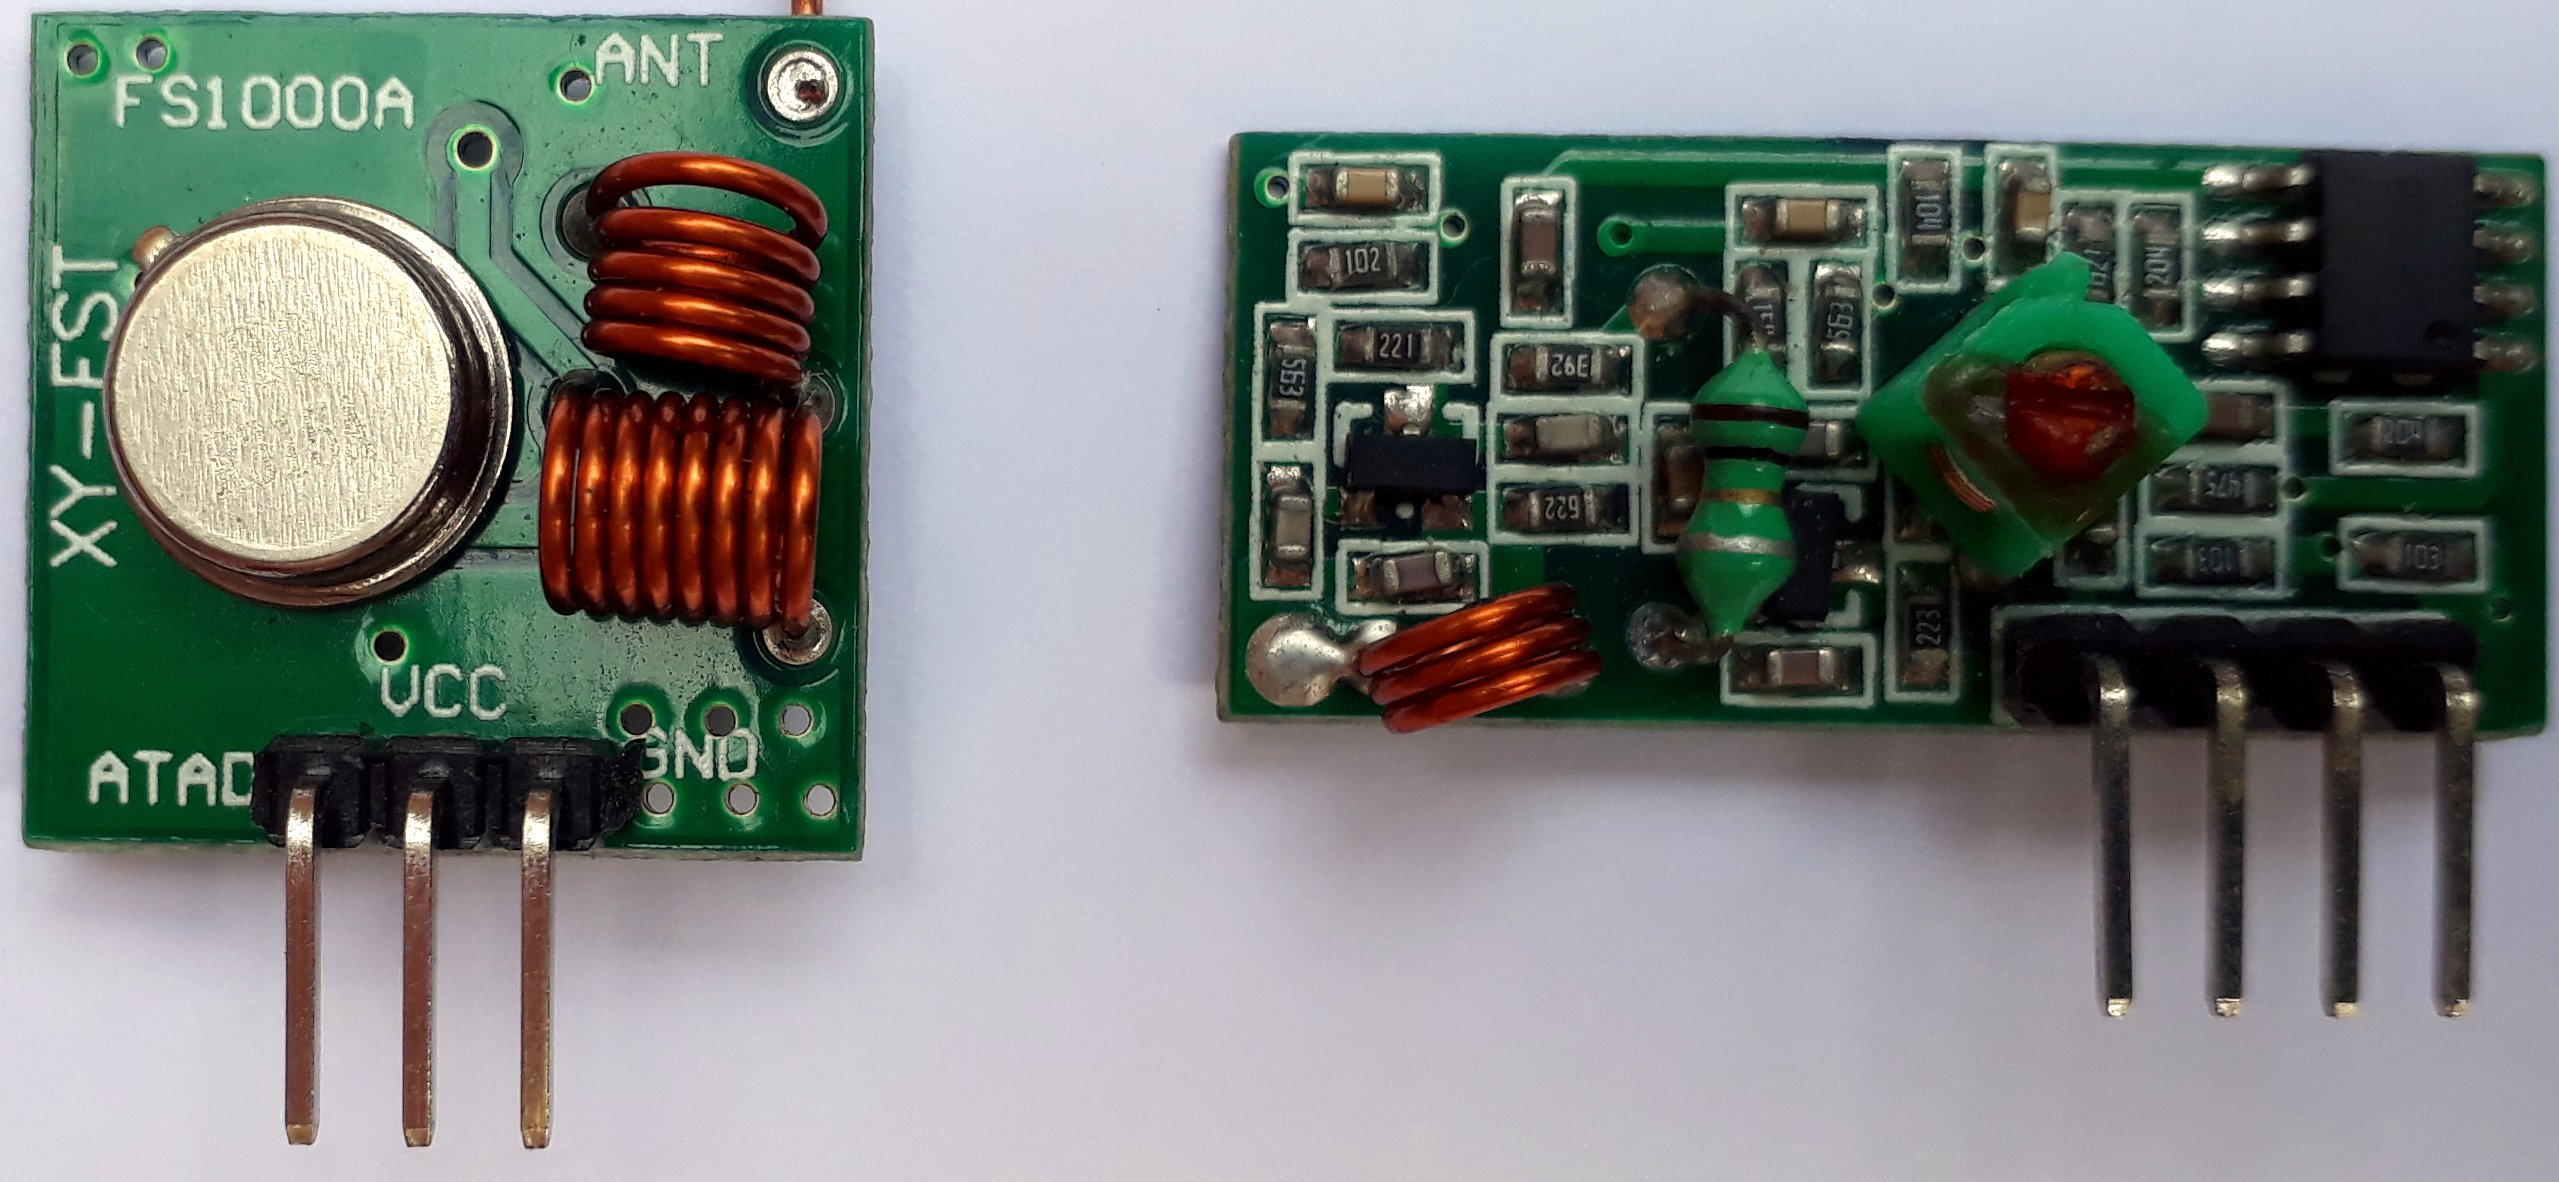
\includegraphics[width=12cm]{./figures/tx-rx1.jpg}
  		\label{Fig:tx-rx1}
			\fonte{Produzido pelo autor.}
		\end{figure}


%+++++++++++++++++++++++++++++++++++++++++++++++++++++++++++++
%
%			TRABALHO PROPRIAMENTE DITO	
%
%+++++++++++++++++++++++++++++++++++++++++++++++++++++++++++++
	
	\chapter{Trabalho Propriamente Dito}

		\section{Introdução}
		
		O capítulo a seguir está organizado em 5 seções. Na primeira delas explica-se a movimentação mecânica do sistema e como as posições de flexão e extensão dos dedos são obtidas pelo microcontrolador. A segunda aborda a programação do microcontrolador, mais precisamente o tratamento dos dados recebidos a partir dos potenciômetros. A terceira seção explica os ajustes realizados em software. A quarta explica o protocolo criado para controlar um carrinho via rádio frequência. A quinta e última seção explica como o sistema foi montado.



		\section{Mecânica Bioinspirada}

			\subsection{Transdutor de Flexão}

		Como foi explicitado previamente, através dos tendões, têm-se a movimentação dos dedos na mão. Baseado nessa biomecânica, foi desenvolvido um sistema mecânico semelhante que visa criar um transdutor de flexão de dedos conectado a um microcontrolador. 

		De uma forma resumida, no sistema natural de movimentação dos dedos, a extremidade do tendão está presa na ponda de uma das falanges do dedo. A extensão do tendão enquanto sua extensão desliza por dentro de polias até o músculo. No sistema desenvolvido, cada transdutor é composto por uma linha de náilon presa ao dedo da luva, guiada através de pequenos segmentos plásticos até o cursor de um potenciômetro. A figura \ref{Fig:bio-and-system} demonstra um pouco dos dois sistemas.


	\begin{figure}[!htb]
		 \centering
		 \caption{(a) Sistema biomecânico e (b) sistema desenvolvido.} 
		 \subfloat[]
		 {
			 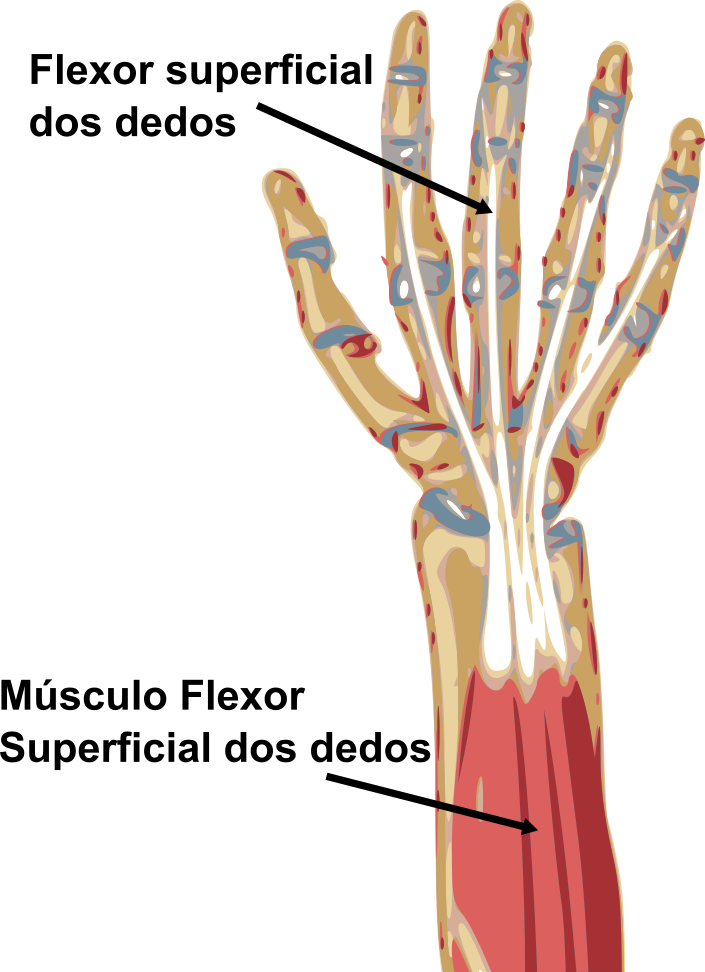
\includegraphics[width=5cm,keepaspectratio=true]{./figures/moore-biomechanic.png}
		 }
		 \centering
		 \subfloat[]
		 { 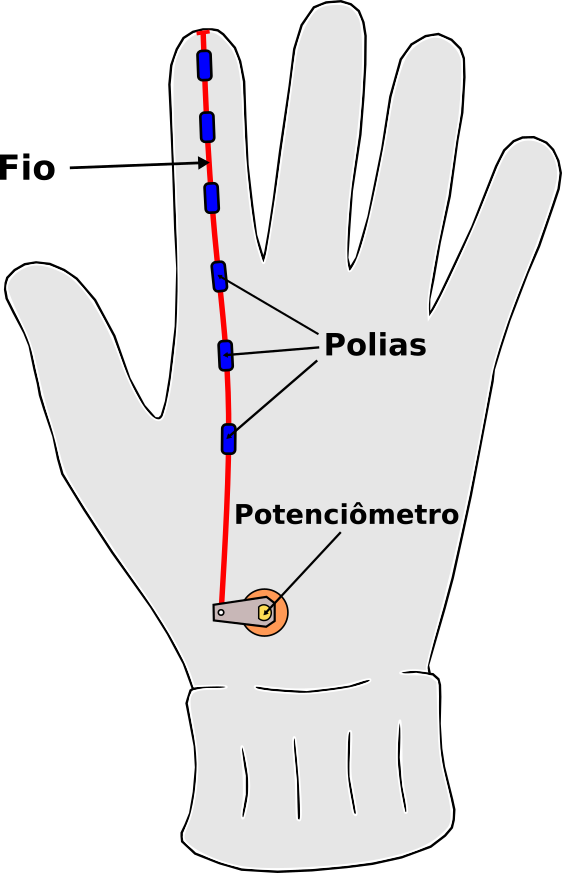
\includegraphics[width=4cm,keepaspectratio=true]{./figures/glove-wire-pot2.png}
		 }
		 \label{Fig:bio-and-system}
		 \fonte{(a) Adaptado de \cite{moore2013clinically} e (b) produzido pelo autor.}
	\end{figure}

		Logo no inicio do trabalho, foi formulada a hipótese de que poderia haver a movimentação de um fio durante a flexão de um dedo. Portanto foi realizado um experimento para verificar tal hipótese. 
		
		Sendo assim, o primeiro passo foi, com a mão inicialmente extendida com o dorso voltado para cima, uma das pontas de um fio foi presa na extremidade de um dos dedos. O local da outra ponta do fio foi marcada no dorso mão. Como é demonstrado na figura \ref{Fig:hand-wire-steady-and-flex} (a).

			Após a flexão dos dedos, verificou-se que o fio se movimentou em uma direção e criou um deslocamento (d) do fio em relação ao ponto marcado, mostrado na figura \ref{Fig:hand-wire-steady-and-flex} (b). Esse experimento validou a hipótese formulada previamente. 

%\begin{figure}[H]
%	\caption{Cabo de pares trançados.}
%	\centering
%	\subfloat[Sem blindagem]{
%		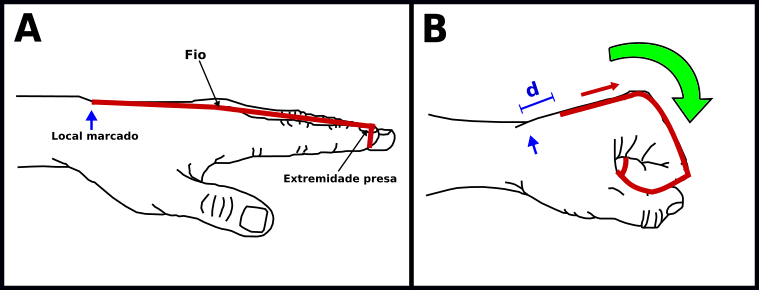
\includegraphics[width=7cm,keepaspectratio=true]{./figures/hand-wire-flex1.png}
%		\label{Fig:UTP}}
 
%	\centering
%	\subfloat[Com blindagem]{
%		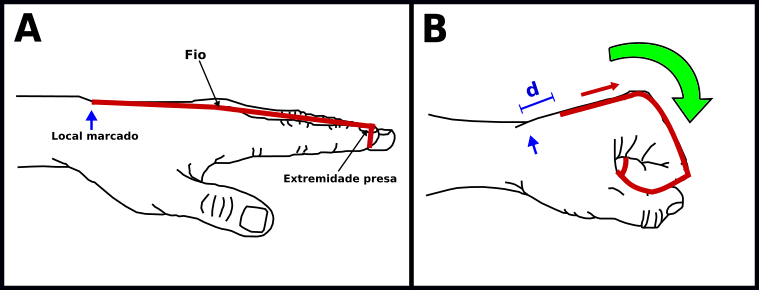
\includegraphics[width=7cm,keepaspectratio=true]{./figures/hand-wire-flex1.png}
%		\label{Fig:STP}}
%	\fonte{.}%
%	\label{Fig:Par}
%\end{figure}

\begin{figure}[!htb]
   \centering
   \caption{ (a) Mão em posição inicial e (b) Mão após flexão.}
   \subfloat[]
   {
     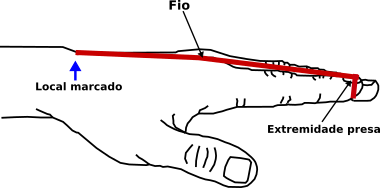
\includegraphics[width=8cm,keepaspectratio=true]{./figures/hand-wire-steady1.png}
   }
   \centering
   \subfloat[]
   { 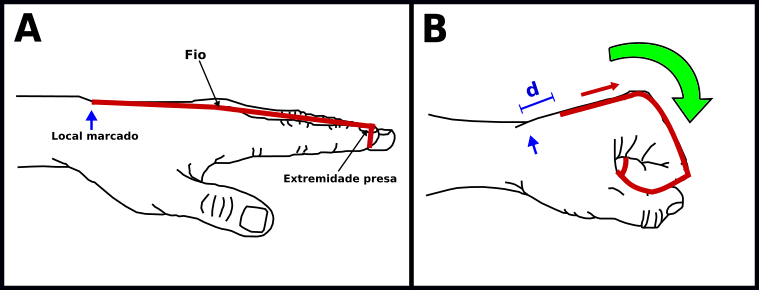
\includegraphics[width=6cm,keepaspectratio=true]{./figures/hand-wire-flex1.png}
   }
   \label{Fig:hand-wire-steady-and-flex}
   \fonte{Produzido pelo autor.}
 \end{figure}


		\subsection{Adaptação na Luva}

%			Após examinar o movimento descrito acima, foi decidido embarcar todo o sistema em uma luva. Fios foram presos às extremidades dos dedos da luva, passando por polias plásticas que servem de guias. Na extremidade oposta, os fios são conectados à pequenos potenciômetros que variam de acordo com o sentido do movimento de cada fio. Figura \ref{Fig:glove-and-transmitter1}. Sendo assim, ao final, para os cinco dedos da mão, serão necessários cinco fios e cinco potenciômetros.


%		\begin{figure}[h!]
%			\centering
%			\caption{Captação do sinal.}
%  		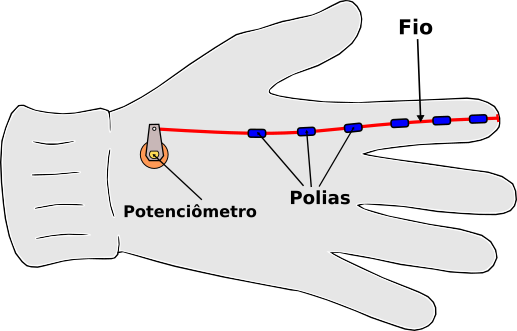
\includegraphics[scale=0.7]{./figures/glove-wire-pot1.png}
%  		\label{Fig:glove-and-transmitter1}
%			\fonte{Produzido pelo autor.}
%		\end{figure}


%		\subsection{Flexão e Extensão dos Dedos}

		Após as polias e o fio de náilon serem devidamente embarcados na luva juntamente ao potenciômetro, com a mão extendida e mantendo o fio de náilon tensionado, ao flexionar o dedo, o fio é puxado pela ponta do dedo e com isso o cursor do potênciometro é variado. Porém, após a flexão do dedo, ao realizar o movimento inverso (extenção), não há força que movimente o fio de náilon e nem o cursor do potenciômetro de volta às suas posições iniciais.
		Para possibilitar que o sistema retorne à sua posição inicial, um pequeno elástico foi instalado junto ao cursor do potenciômetro. Usando o elástico durante o movimento de flexão, o cursor gira e estica o elástico. Estando esticado, o elástico busca retomar sua posição de equilíbro realizando uma força contrária para girar o cursor de volta à sua posição inicial. Figura \ref{Fig:glove-flex-and-extend2} (a).		
		Quando há o movimento de extensão do dedo, o elástico puxa o cursor do potenciômetro girando-o em sentido inverso ao que ocorreu durante a flexão. Isso acontece enquanto o elástico estiver esticado o suficiente para exercer força sobre o cursor do potenciômetro. Demonstrado na figura \ref{Fig:glove-flex-and-extend2} (b)
		

	\begin{figure}[!htb]
		 \centering
		 \caption{ Movimentos da luva de (a) flexão e (b) extensão.} 
		 \subfloat[]
		 {
			 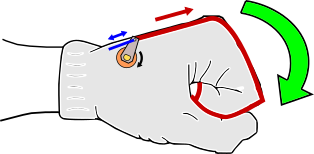
\includegraphics[width=6.5cm,keepaspectratio=true]{./figures/glove-wire-flex2.png}
		 }
		 \centering
		 \subfloat[]
		 { 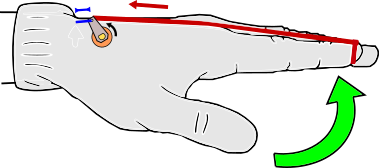
\includegraphics[width=7.5cm,keepaspectratio=true]{./figures/glove-wire-extend2.png}
		 }
		 \label{Fig:glove-flex-and-extend2}
		 \fonte{Produzido pelo autor.}
	\end{figure}


	
		\section{Programação do microcontrolador}

		\subsection{Digitalização do sinal}

		Na luva, além do transdutor, há um microcontrolador que capta os movimentos do potenciômetro e os digitaliza. O sinal chega em portas analógicas de um Arduino modelo Nano que converte a variação de tensão do potenciômetro em valores inteiros entre 0 e 1023. 

		Para facilitar a abordagem do trabalho, cada dedo da luva e seu respectivo potenciômetro é representado por um número de 1 a 5, começando pelo dedo mínimo (1) até o polegar (5). 
	 Também foram definidas duas posições principais para analisar o movimento dos dedos. Posição A: Quando todos os dedos estiverem estendidos. Posição B: Quando todos os dedos estiverem flexionados. Algo semelhante à figura \ref{Fig:glove-flex-and-extend2}.

	 	Para cada posição, o potenciômetro apresenta uma média de valores digitais. Por exemplo, quando o dedo mínimo (1) está extendido (posição A), seu respectivo potenciômetro apresenta valores em torno 191. Quando esse dedo é totalmente flexionado (posição B) seus valores ficam em torno de 616. %Então para calcular o deslocamente temos:

%	\begin{equation}
%		\begin{split}
%			\Delta Pos 	& = Pos 2 	- 	Pos 1 	\\
%									& = 558 		- 	157			\\
%						 			& = +383
%		\label{Eq:Desloca1}
%		\end{split}
%	\end{equation}

		Porteriormente, para diminuir o tamanho da mensagem a ser enviada, o valor digital apresentado pelo potenciômetro é remapeado para uma faixa de valores inteiros que representam posições inteiras entre 0 e 9. Quando os valores de todos os potenciômetros são remapeados, eles são concatenados em um único número de 5 dígitos, no qual cada dígito representa cada um dos cinco dedos da esquerda para a direita. 
		
		Por exemplo, em uma mensagem "69071" o dedo 1 (mínimo) está na posição 6, o dedo 2 (anelar) está na posição 9 e assim sucessivamente até o dedo 5 (polegar) que está na posição 1.
		
		
		\subsection{VirtualWire}

		VirtualWire é uma biblioteca de comunicação para Arduino que possibilita vários Arduinos se comunicarem usando transmissores e receptores RF de baixo custo. Essa biblioteca permite o envio de mensagens curtas, sem endereçamento, retransmissão ou confirmação, como se fosse uma espécie de protocolo UDP (\textit{User Datagram Protocol}), usando modulação ASK (\textit{Amplitude Shift Keying}) \cite{virtualwiremanual}. 

		O uso dessa biblioteca nos códigos da IDE do Arduino, permite abstrair tratamentos de envio e recebimento de dados tais como, sincronização de padrões, balanceamento de bits 0 e 1, e checagem de erros \cite{virtualwirepjrc}. Dessa forma, para enviar e receber mensagens, basta seguir os padrões de entrada e saída das funcões descritas na biblioteca.

		No código embarcado no microcontrolador da luva foram definidos, segundo os parâmetros da biblioteca, o pino do transmissor RF, a taxa de transmissão e o tamanho da mensagem a ser enviada. Porém, antes de efetivamente enviar a mensagem é preciso convertê-la em uma string que logo em seguida será transformada em um vetor de char, que é o formato de dado aceito pela função de envio.

		Uma das formas de converter valores inteiros em string é concatenar o valor inteiro com uma string \cite{arduinostringadd}. Por isso, no código desenvolvido, uma string vazia é somada aos valores inteiros remapeados dos potenciômetros. Com isso, os valores serão concatenados e transformados em uma string ao mesmo tempo. Essa string então é transformada em um vetor de char usando a função "toCharArray" antes de ser enviada. Este processo está descrito resumidamente no pseudocódigo abaixo.		

\lstset{language=C++,
%                basicstyle=\ttfamily,
                keywordstyle=\color{blue}\ttfamily,
                stringstyle=\color{green}\ttfamily,
                commentstyle=\color{red}\ttfamily,
								basicstyle=\footnotesize,
                morecomment=[l][\color{magenta}]{\#}
}
\begin{lstlisting}
	// Inicia variaveis
	string vazia = ""
	string mensagem = ""
	
	// Recebe as posicoes de cada dedo
	int dedo1 = posicao_dedo1;
	int dedo2 = posicao_dedo2;
	int dedo3 = posicao_dedo3;
	int dedo4 = posicao_dedo4;
	int dedo5 = posicao_dedo5;

	// Concatena os inteiros e os transforma em string
	mensagem = vazia + dedo1 + dedo2 + dedo3 + dedo4 + dedo5;

	// Converte a string em um vetor de char
	mensagem = mensagem.toCharArray;

	// Envia o vetor de char
	vw_send(mensagem);

\end{lstlisting}

				
%		Um resumo do processo de digitalização e envio é demonstrado na figura \ref{Fig:get-and-send}.


%		\begin{figure}[h!]
%			\centering
%			\caption{Digitalização e envio do sinal}
%  		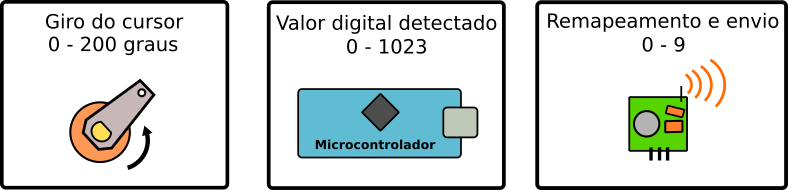
\includegraphics[width=12cm]{./figures/get-and-send.png}
% 		\label{Fig:get-and-send}
%			\fonte{Produzido pelo autor.}
%		\end{figure}



		\section{Ajustes}
		
		\subsection{Introdução}

		Quando os dedos estão em um mesmo grau de flexão, na grande maioria das vezes, os valores detectados para cada dedo são diferentes. Quando a luva está em posição A (extendida), por exemplo, o valor detectado no dedo mínimo (1) fica em torno de 192, enquanto que o anelar (2) apresenta, ao mesmo tempo, um valor em torno de 141.	
		
		Além do mais, devido à posição em que cada potenciômetro foi soldado na placa embarcada, alguns potênciômetros apresentam deslocamentos positivos ou negativos para um mesmo movimento. 
	
		\subsection{Deslocamento e número de posições}

		Para descobrir os valores de deslocamento, cada potenciômetro teve seu valor digital anotado para as posições A e B, que posteriormente foram usados na equação \ref{Eq:Desloca1}:

	\begin{equation}
			\Delta Pos 	= Pos B 	- 	Pos A
		\label{Eq:Desloca1}
	\end{equation}

		Usando o módulo de $\Delta Pos$ é possível calcular o número de posições detectáveis partindo da Posição A até a Posição B, através da equação \ref{Eq:NPos1}:

	\begin{equation}
			NPos = |\Delta Pos| + 1
		\label{Eq:NPos1}
	\end{equation}

		A tabela \ref{Tab:deltapos} mostra os valores obtidos e calculados para cada um dos cinco potenciômetro no deslocamento da posição A para a posição B.


	\begin{table}[H]
  	\centering
		\caption{Valores de A para B}
    \begin{tabular}{c|cccc}
      \midrule
			Dedo	& PosA	& PosB	& $\Delta$Pos	& NPos	\\
      \midrule
			1 		& 191 	& 616 	& 		+425 		&	426		\\
			2 		& 140 	& 609 	& 		+469 		&	470		\\
			3 		& 774 	& 360 	& 		-414 		&	415		\\
			4 		& 728 	& 475 	& 		-253 		&	254		\\
			5 		& 670 	& 367 	& 		-303 		&	304		\\      
      \midrule
    \end{tabular}
    \label{Tab:deltapos}
    \fonte{Produzido pelo autor}
	\end{table}
		
		Quanto maior for o valor de NPos na tabela \ref{Tab:deltapos}, mais preciso será o sensoriamento do dedo. Sendo assim, o anelar (2) é o dedo com maior potencial de sensoriamento, enquanto que o indicador (4) possui menor potencial.

	\subsection{Remapeamento}

	 Com o intuito de diminur o tamanho da mensagem a ser enviada pelo transmissor de rádio frequência, foi definido que cada potenciômetro teria apenas 10 níveis de deslocamento representados durante a transmissão. Dessa forma, em uma mensagem numérica, bastaria 1 dígito para representar a posição atual do dedo.

	 Junto a isso, para diminuir a complexidade do protocolo de comando, foi decidido que não haveriam deslocamentos negativos. Algo que acontece nos dedos 3, 4 e 5 durante o deslocamente de A para B.

	 Para se adequar aos requisitos descritos, no código embarcado foi usada a função "map", que permite remapear uma faixa de valores em outra menor. Usando tal função, a faixa de entrada que inicialmente poderia variar entre 0 e 1023, foi remapeada para variar entre 0 e 9 valores inteiros. 
	 
	 Além do mais, a função map também permite inverter a saída, de uma forma que os valores de entrada que variam de 1023 a 0 (decrescente) passarão a variar de 0 a 9 (crescente). Este último requisito, permite eliminar os deslocamentos negativos.

	 Usando as equações \ref{Eq:Desloca1} e \ref{Eq:NPos1}, os valores digitais remapeados (R) foram adicionados à tabela \ref{Tab:deltapos}, criando a tabela \ref{Tab:deltaremap}:


	\begin{table}[H]
  	\centering
		\caption{Valores de A para B e remapeados (R).}
    \begin{tabular}{c|cc|cc|cc|cc}
      \midrule
			Dedo	&\multicolumn{2}{c}{PosA	(RA)} 	&\multicolumn{2}{c}{PosB (RB)}	&\multicolumn{2}{c}{$\Delta$Pos	($\Delta$R)}	&\multicolumn{2}{c}{NPos	(NR)}	\\
      \midrule
			1 		& 191 & (1)		& 616 & (5)		& 		+425 & (+4)		&			425	& (5)		\\
			2 		& 140 & (1)		& 609 & (5)		& 		+469 & (+4)		&			469 &	(5)		\\
			3 		& 774 & (3)		& 360 & (6)		& 		-414 & (+3)		&			414	& (4)		\\
			4 		& 728 & (3)		& 475 & (5)		& 		-253 & (+2)		&			253	& (3)		\\
			5 		& 670 & (4)		& 367 & (6)		& 		-303 & (+2)		&			303 &	(3)		\\      
      \midrule
    \end{tabular}
    \label{Tab:deltaremap}
    \fonte{Produzido pelo autor}
	\end{table}
	

		
		\section{Protocolo de comunicação}

		\subsection{Introdução}

		Através de um transmissor de rádio frequência, a o sistema embarcado na luva envia constantemente mensagens de 5 dígitos que indicam a posição de cada um dos cinco dedos. Para receber esse sinal, é preciso usar um módulo receptor de rádio frequência compatível com o transmissor. 
		
		Um sistema receptor foi embarcado em um carrinho usando um segundo microcontrolador Arduino modelo Nano e um módulo receptor RF. Esse carrinho funciona com motores DC (\textit{Direct Current}) e todo o sistema é alimentado por uma bateria LiPo. 

		Para possibilitar o controle, conjuntos pré-definidos das posições dos dedos correspondem a movimentos que devem ser executados pelo carrinho.
		
		\subsection{Posições e movimentos}

		Como foi explicitado anteriormente, a mensagem transmitida pela luva consiste em um conjunto de 5 dígitos no qual cada dígito indica a posição de um respectivo dedo. Na mensagem, o primeiro dígito da esquerda indica a posição do dedo 1, que é o dedo mínimo. O segundo dígito indica a posição do dedo 2, ou seja, o dedo anelar. Essa lógica segue até o quinto dígito que representa a posição do dedo polegar.

		Cinco comandos foram definidos para o carrinho, ir para frente, ir para trás, girar para a esquerda, girar para a direita e parar. Com o intuito de controlar o carrinho através de combinações de flexões e extensões de dedos, 5 conjuntos de posições também foram definidas. São eles: flexionar os dedos 2 e 3 simultanemanete, flexionar somente o dedo 4, flexionar somente o dedo 5, flexionar apenas o dedo 1 e não flexionar nenhum dedo.

		A figura \ref{Fig:glove-control-positions1} mostra a correspondência entre cada combinação de flexão dos dedos e seu respectivo comando para o carrinho. Apenas os dedos indicados em vermelho devem ser flexionados para validar o comando. Qualquer outra combinação faz o carrinho parar.


		\begin{figure}[h!]
			\centering
			\caption{Comandos a partir de flexões e extensões para controle do carrinho}
  		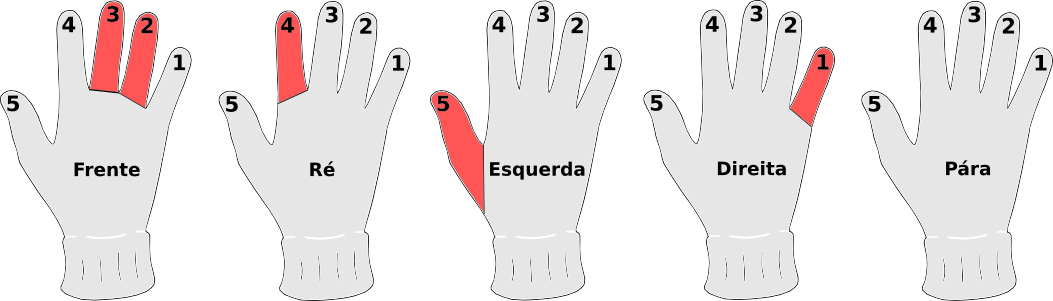
\includegraphics[width=14cm]{./figures/glove-control-positions1.png}
  		\label{Fig:glove-control-positions1}
			\fonte{Produzido pelo autor.}
		\end{figure}

		
		\subsection{\textit{Software} de recepção}

		A biblioteca VirtualWire também deve estar presente no código do microcontrolador embarcado no carrinho. Para receber as mensagens adequadamente, é necessário definir o pino do receptor RF e indicar a taxa de transmissão do transmissor RF. Também deve-se criar variáveis para guardar a mensagem recebida e o seu tamanho, pois as mensagens são recebidas \textit{byte} a \textit{byte}.

		Uma função nativa da biblioteca verifica se chegou alguma mensagem e indica \textit{true} quando isso acontece. Então, ao receber uma mensagem, para lê-la, é necessário criar um \textit{for} que recebe como parâmetro o tamanho da mensagem recebida. Dentro da função a mensagem será lida \textit{byte} a \textit{byte} enquanto a função \textit{for} for verdadeira.

		O pseudocódigo abaixo demonstra o fluxo descrito:


\begin{lstlisting}
	// Define as variaveis
	int pino_receptor = 8;
	int taxa_transmissao = 2000;
	
	// Recebe a mensagem e o seu tamanho
	byte msg = get_mensagem;
	byte tamanho_msg = get_tamanho_msg;
	
	// Aguarda receber alguma mensagem
	chegou_mensagem = vw_wait_rx();

	// Verifica se ha mensagem, inicia o for para ler cada byte
	if(chegou_mensagem){
		for (int i = 0; enquanto i < tamanho_msg; i++)
			byte_recebido[i] = msg[i];		
	}
\end{lstlisting}

		Usando o pseudocódigo apresentado e sabendo que na mensagem recebida o primeiro dígito indica a posição atual do dedo 1, percebe-se que a função \textit{for} irá rodar pelo menos 5 vezes, armazenando em cada posição do vetor \texttt{byte\_recebido[]} as informações de cada dedo. Dessa maneira, a posição recebida do dedo 1 estará em \texttt{byte\_recebido[0]}, enquanto que a do dedo 2 está em \texttt{byte\_recebido[1]}. Continuando assim até o dedo 5 que estará em \texttt{byte\_recebido[4]}.
		
		Após o armazenamento das posições dos dedos, cinco funções foram criadas para comandar a ponte H e dessa forma movimentar os motores do carrinho. São elas: FRENTE( ), TRAS( ), ESQUERDA( ), DIREITA( ) e PARA( ). Ao chamar qualquer uma dessas funções, o carrinho passa a se movimentar na direção e sentido definidas.
		Para chamar a função correta baseada na mensagem recebida, foram criadas cadeias de \textit{Ifs} e \textit{Elses} nas quais, quando satisfeitas certas condições, a respectiva função é chamada. 
		
		A tabela \ref{Tab:dedos-e-comandos1} mostra quais são os conjuntos de valores esperados para todos os dedos simultaneamente em cada comando. Ou seja, para saber qual a combinação de valores para movimentar o carrinho para frente, é só observar a coluna "Frente" da tabela. Qualquer outra combinação além das especificadas na tabela, fará o carrinho ficar parado. Os dedos flexionados estão destacados em vermelho.

		\begin{table}[H]
     \centering
     \caption{Valores recebidos dos dedos e comandos de movimento}
     \begin{tabular}{c|ccccc}
			 \midrule
			 Dedo &       Frente			 & 				Tras				& 		Esquerda			 & 		Direita					& Para	\\
			 \midrule
			 1    & < 2   						 & < 2   							& < 2    						 &\textcolor{red}{> 1}&	-			\\
			 2    &\textcolor{red}{> 1}& < 2   							& < 2  	 						 & < 2   							&	-			\\
			 3    &\textcolor{red}{> 3}& < 4   							& < 4   						 & < 4   							&	-			\\
			 4    & < 4   						 &\textcolor{red}{> 3}& < 4 							 & < 4   							&	-			\\
			 5    & < 5   						 & < 5   							&\textcolor{red}{> 4}& < 5   							&	-			\\
			 \midrule
     \end{tabular}
     \label{Tab:dedos-e-comandos1}
     \fonte{Produzido pelo autor}
   \end{table}



%		Para poder controlar o carrinho, foi necessário criar um protocolo de comunicação que traduzisse os movimentos de flexão dos dedos em comandos e direções para o carrinho que receberia o sinal.


		\section{Montagem do protótipo}

		\subsection{Transdutor de Flexão}

		A escolha de materiais foi baseada no menor custo e maior disponibilidade local. Prevendo a possibilidade de costuras no projeto, um par de luvas de algodão foi escolhida. O sistema foi embarcado na luva direita, enquanto que a esquerda poderia ser usada em caso de dano da primeira.
		
		As polias plásticas são feitas a partir de pequenos pedaços de hastes flexíveis com algodão nas pontas. Sendo que apenas a parte plástica foi aproveitada enquanto que o algodão foi descartado.

		O material da linha que movimenta os cursores dos potenciômetro é náilon por sua boa resistência e durabilidade, além de aparentar ter pouca ou nenhuma elasticidade para a aplicação.

		Utilizando a luva escolhida com o dorso voltado para cima, as polias plásticas foram costuradas ao longo dos dedos. Uma das extremidades de cada fio de náilon foi presa na ponta de cada um dos dedos, enquanto que o restante do fio passava por dentro das polias plásticas. A outra extremidade do fio de náilon seria amarrada ao cursor do potenciômetro quando a PCB fosse incluída na luva. A figura \ref{Fig:glove-wire-pot1} demostra o resultado esperado para um dos dedos da luva.


		\begin{figure}[h!]
			\centering
			\caption{Costura do transdutor em um dedo.}
  		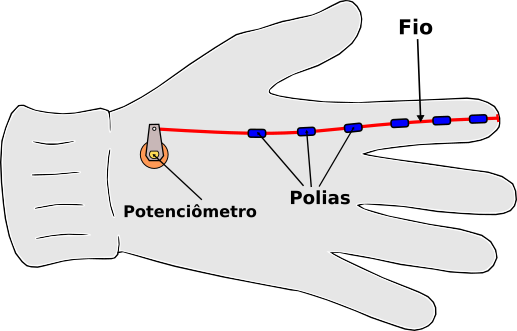
\includegraphics[width=7cm]{./figures/glove-wire-pot1.png}
  		\label{Fig:glove-wire-pot1}
			\fonte{Produzido pelo autor.}
		\end{figure}

			
			\subsection{Escolha de componentes}	

			O sistema de processamento e transmissão de sinal embarcado na luva, foi projetado para ser móvel, leve, alimentado por uma bateria, caber no dorso da mão e ter custo relativamente menor em relação à soluções com sensores flex tradicionais. O sistema deve ser de fácil reprodução e o mais adaptável possível à outras formas de transmissão além da rádio frequência, caso estas sejam necessárias futuramente.

			O primeiro desafio foi escolher, dentre os componentes disponíveis, quais seriam utilizados para compor a eletrônica presente na placa de circuito impresso que estaria embarcada na luva.

			O potenciômetro foi o primeiro componente a ser definido. Isso porque, este seria o componente  em maior número na placa. O modelo escolhido deveria ser pequeno suficiente para manter uma distância adequada para outros potenciômetros e componentes. Seu cursor deveria ser de fácil giro, para que pudesse ser acionado apenas pelo deslocamento do fio. Seu ângulo de giro total precisava ser mínimo, para que o menor grau de giro correspondesse à maior variação de resistência possível, facilitando assim a percepção pelo microcontrolador.

			O modelo de potenciômetro que mais se aproximou das especificações acima foi retirado de servomotores modelo MG996R da marca TowerPro. O potenciômetro encontrado possui dimensão aproximada de 13$\,mm$ x 13$\,mm$, resistência máxima de 5$\,$k$\Omega$, giro máximo de $200^{o}$ (aproximado) e oferece pouca resistência para girar seu cursor. 

			Um pequeno pedaço de PVC (\textit{Polyvinyl Chloride}) expandido foi adaptado ao cursor do potenciômetro para facilitar o seu giro, amarrar uma das extremidades do fio de náilon e para prender um elástico. Essa adaptação pode ser vista na figura \ref{Fig:potentiometer-and-battery}.a.

			O microcontrolador escolhido para processar os dados recebidos de cada potenciômetro foi o Arduíno modelo Nano. Isso porque ele é leve, ocupa uma área de apenas 45$\,mm$ x 17$\,mm$, possui vasta documentação e disponibilidade no mercado, além de ser compatível com diversos módulos externos e possuir custo menor do que outros modelos da família Arduino.

			Para transmitir e receber o sinal, foi escolhido o par de RF 433$\,MHz$, que é leve e de baixo custo comparado à outras soluções de transmissão de dados.

			Finalmente, para alimentar esse aparato eletrônico, foi escolhida uma pequena bateria LiPo (\textit{Lithium-ion Polymer}) que possui capacidade de 300$\,mAh$, 7,4$\,V$ de tensão nominal e ocupa um espaço de 45$\,mm$ x 12,5$\,mm$. Esse modelo é mostrado na figura \ref{Fig:potentiometer-and-battery}.b.


	\begin{figure}[!htb]
		 \centering
		 \caption{ (a) Potenciômetro adaptado e (b) bateria.}
		 \subfloat[]
		 {
			 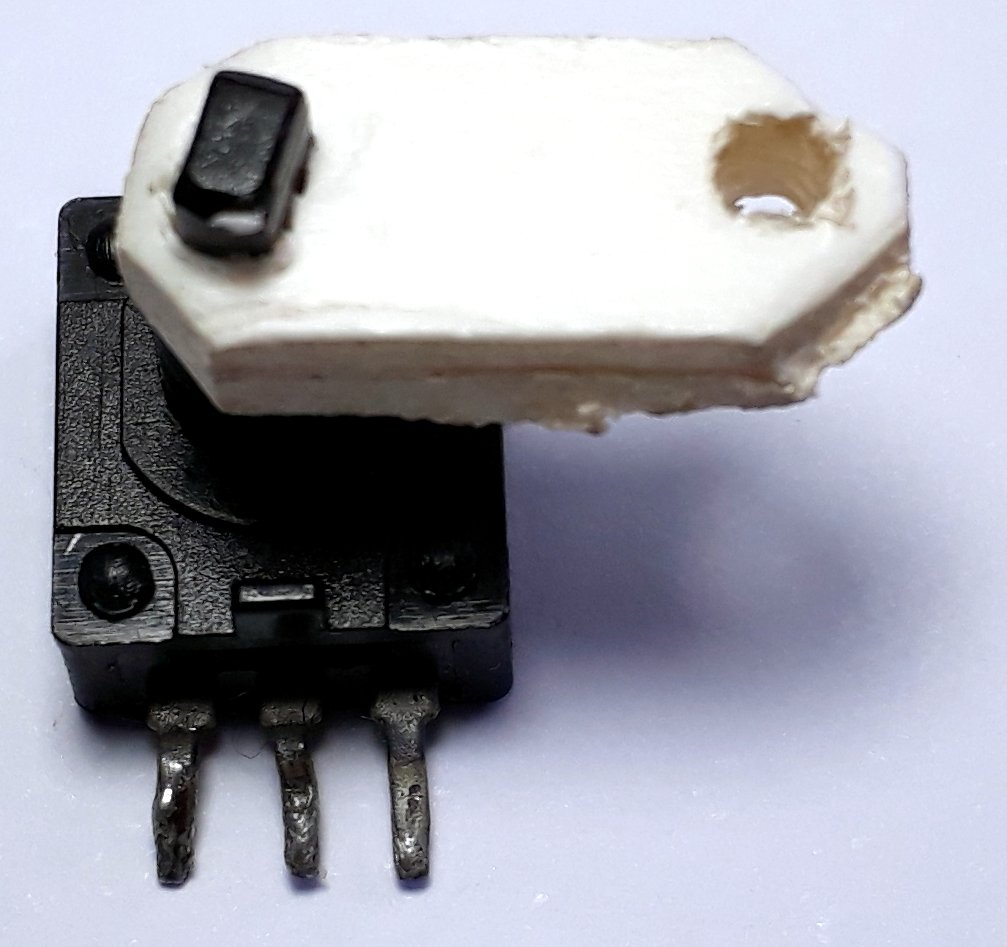
\includegraphics[width=5.5cm,keepaspectratio=true]{./figures/potentiometer3.jpg}
		 }
		 \centering
		 \subfloat[]
		 { 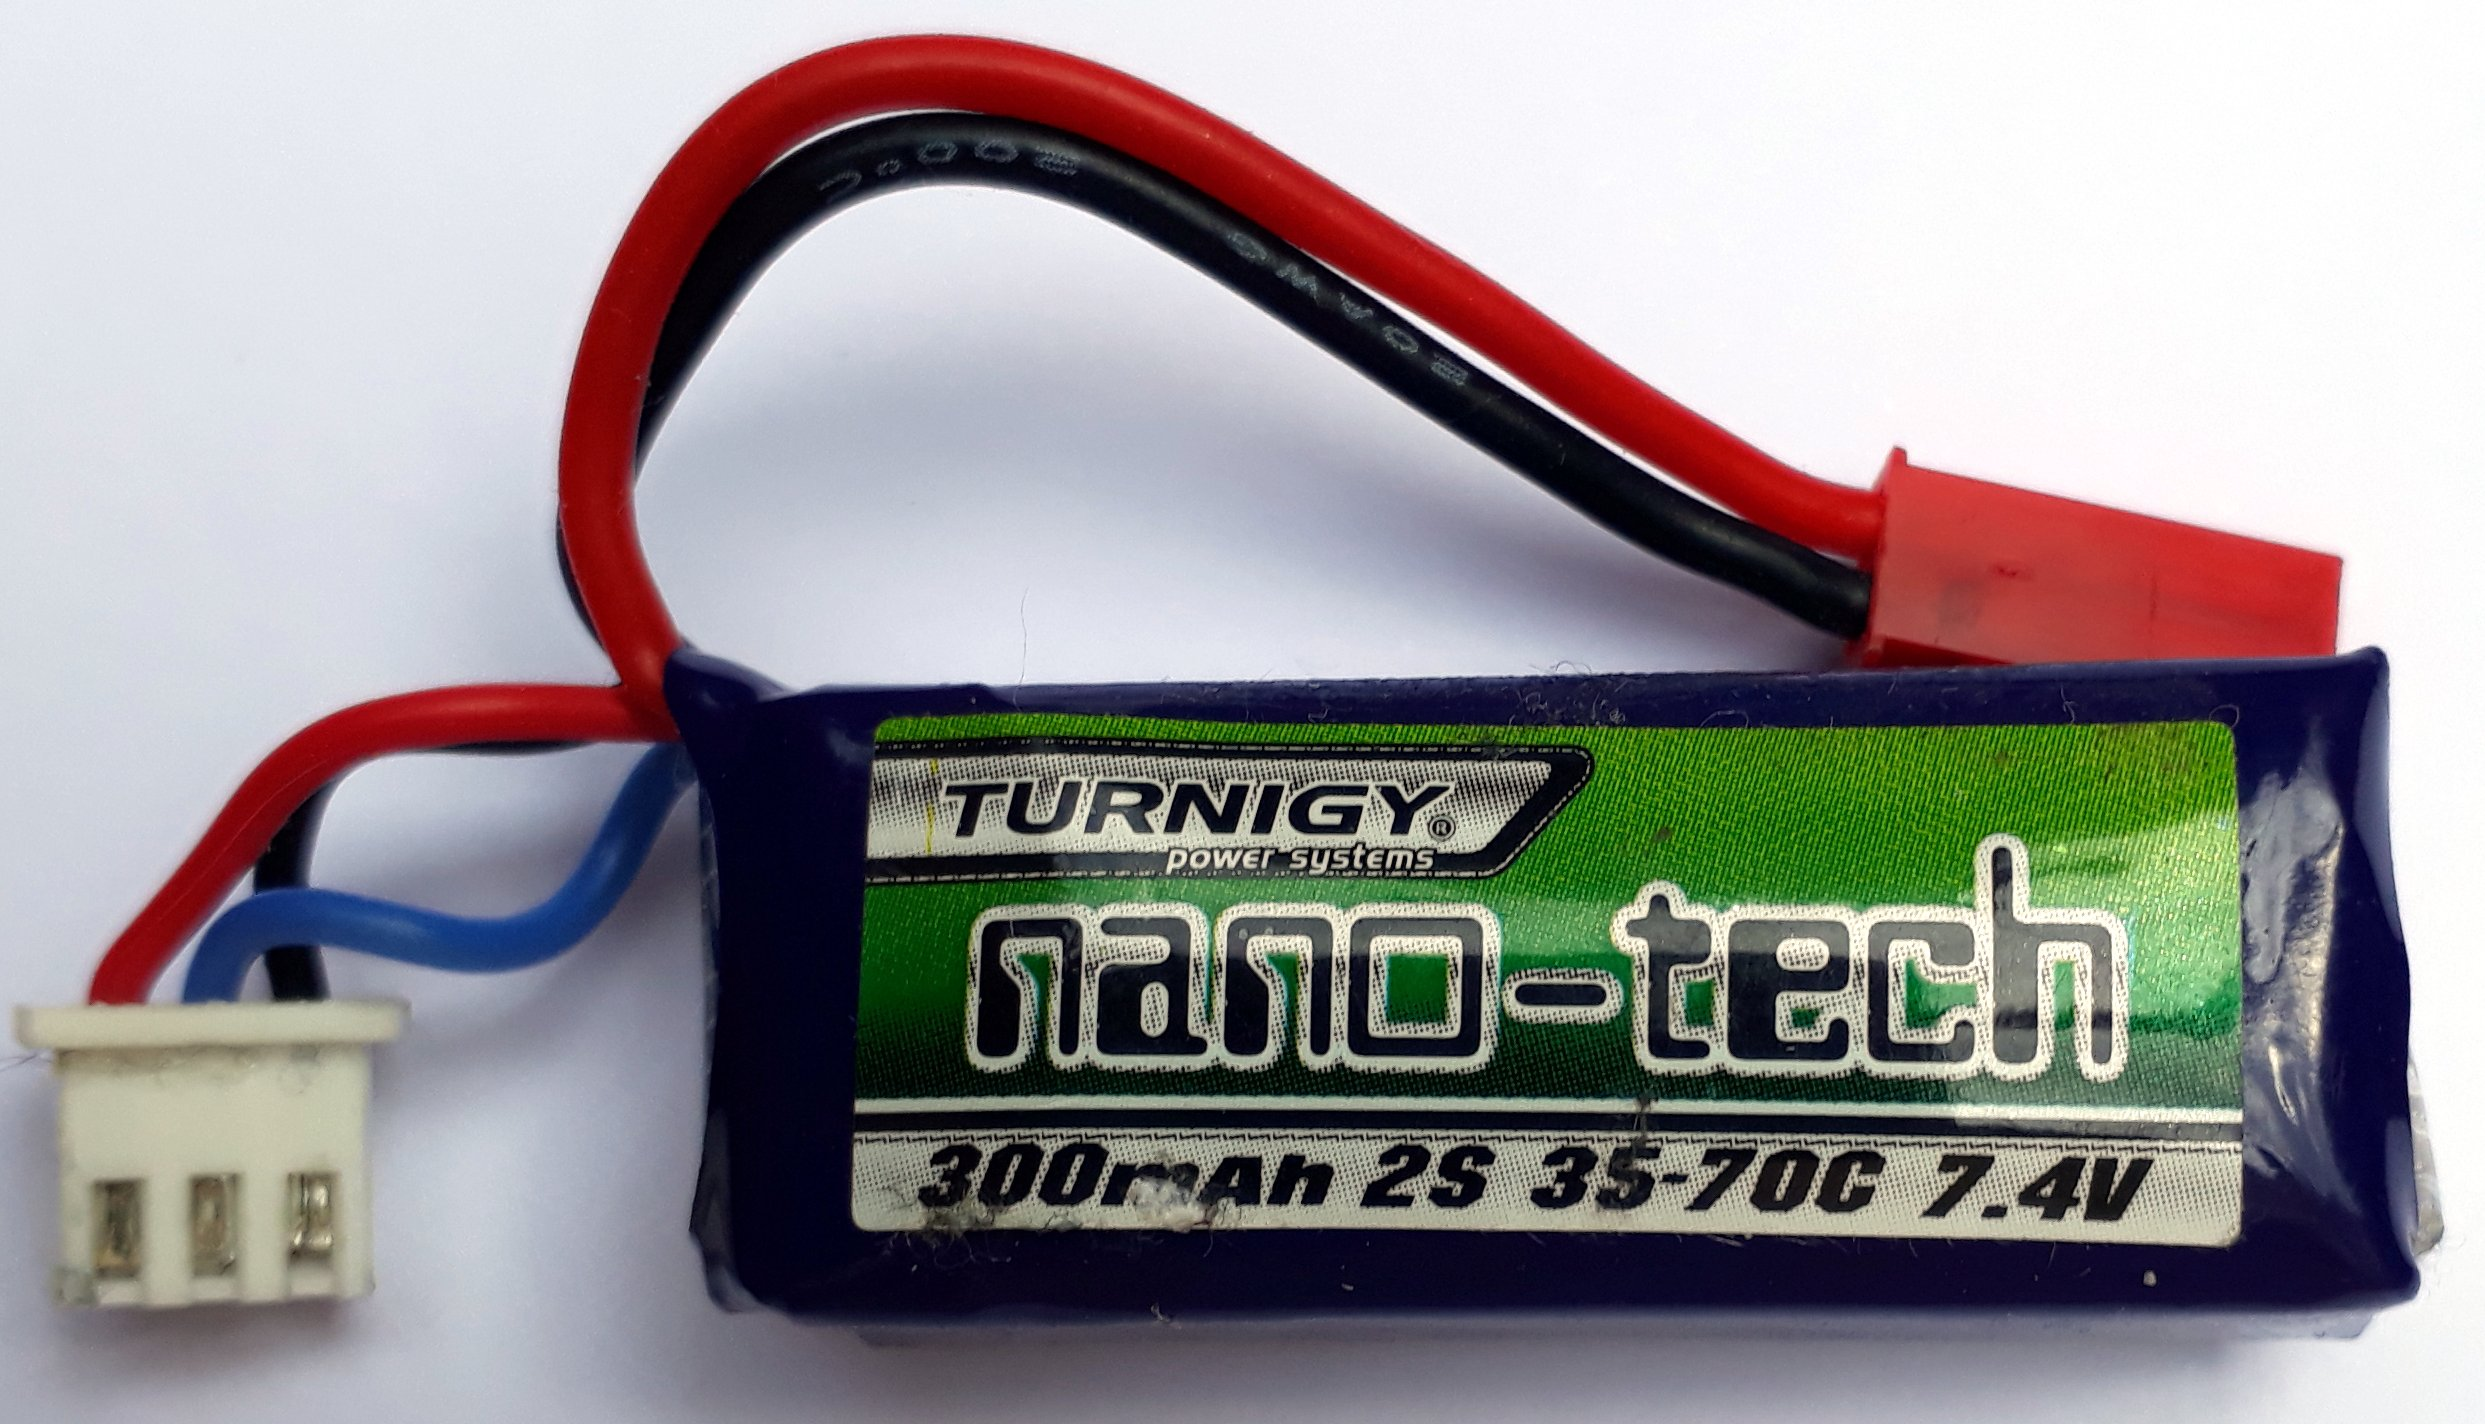
\includegraphics[width=8.5cm,keepaspectratio=true]{./figures/battery1.jpg}
		 }
		 \label{Fig:potentiometer-and-battery}
		 \fonte{Produzido pelo autor.}
	 \end{figure}


			\subsection{Posicionamento de componentes}

			Após medições realizadas na luva que serviu de modelo para o projeto, foi decidido que a dimensão máxima da PCI (Placa de Circuito Impresso) deveria ser de aproximadamente 72$\,mm$ x 58$\,mm$, para que a placa não ficasse muito maior do que o dorso da luva. Sendo assim, usando o software QCAD, todos os componentes foram organizados dentro da placa basendo-se nas suas dimensões aproximadas. O \textit{layout} final da placa é apresentado na figura \ref{Fig:size-glove-module1}.

		\begin{figure}[h!]
			\centering
			\caption{Dimensões aproximadas da PCI e seus componentes.}
  		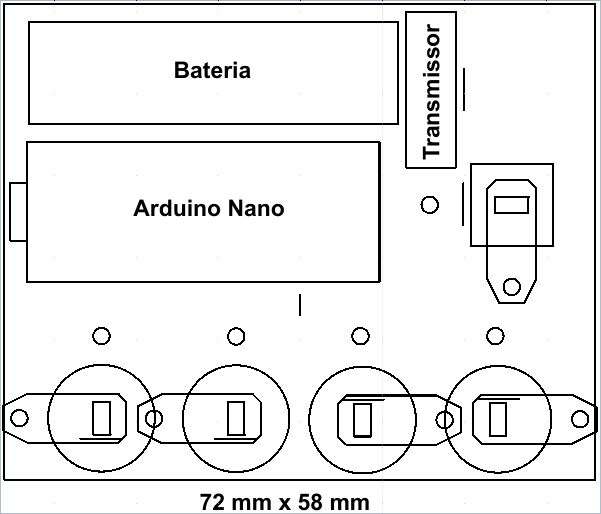
\includegraphics[width=7cm]{figures/size-glove-module1.png}
  		\label{Fig:size-glove-module1}
			\fonte{Produzido pelo autor.}
		\end{figure}


			\subsection{Placa Embarcada}

			Os primeiros experimentos de comportamento e ligação entre os componentes foram realizados ainda em protoboard. Inicialmente, um programa lia a variação de um resistor e mostrava na tela do computador. Este e outros programas foram usados para verificar como deveriam ser as conexões entre os pinos, potenciômetros, bateria, módulo transmissor e o microcontrolador Arduíno.

			O passo seguinte foi utilizar o software gratuito Kicad para desenhar o esquemático da placa. Posteriormente, o Kicad ainda possibilita projetar uma placa de circuito impresso baseada no esquemático desenhado anteriormente. Através desse software foram criados os desenhos do esquemático e da PCI embarcada mostrados na figura \ref{Fig:schematic-and-PCB}.

	\begin{figure}[!htb]
		 \centering
		 \caption{ Desenhos projetados no Kicad do (a) esquemático e (b) PCI. }
		 \subfloat[]
		 {
			 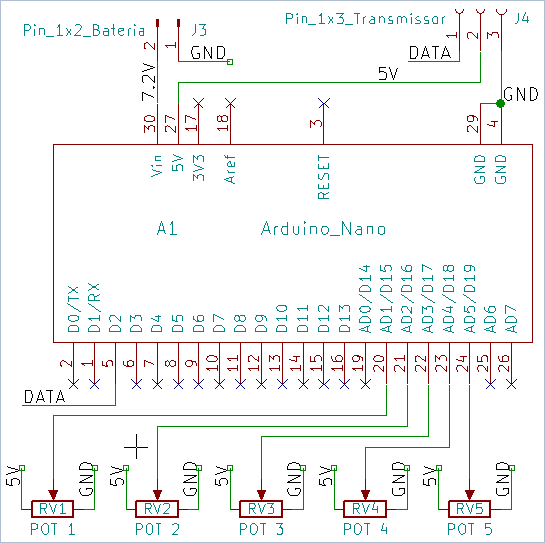
\includegraphics[width=6.5cm,keepaspectratio=true]{./figures/schematic-glove-module1.png}
		 }
		 \centering
		 \subfloat[]
		 { 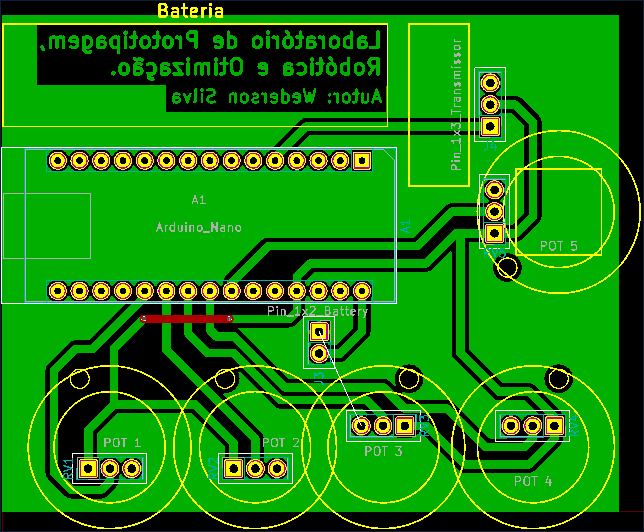
\includegraphics[width=7.5cm,keepaspectratio=true]{./figures/PCB-glove-module1.png}
		 }
		 \label{Fig:schematic-and-PCB}
		 \fonte{Produzido pelo autor.}
	\end{figure}

			Após a conclusão do desenho da placa, foram efetuados os procedimentos necessários para a confecção desta PCI em uma placa de fenolite cobreada, além da posterior soldagem de pinos e componentes. A figura \ref{Fig:phenolic-and-ready} mostra os resultados após o procedimento descrito. Já a figura \ref{Fig:glove-ready1} mostra o resultado final após juntar a luva de algodão e a placa de circuito impresso recém concluída.

	\begin{figure}[!htb]
		 \centering
		 \caption{(a) Placa de fenolite cobreada e (b) com os componentes soldados.} 
		 \subfloat[]
		 {
			 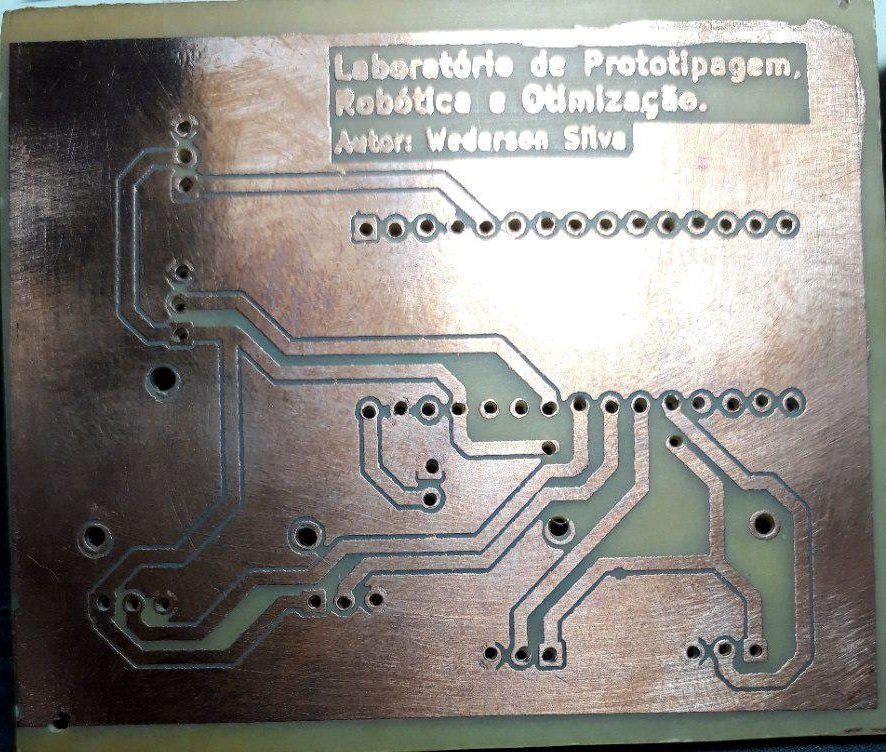
\includegraphics[width=7cm,keepaspectratio=true]{./figures/phenolic-glove-module1.jpg}
		 }
		 \centering
		 \subfloat[]
		 { 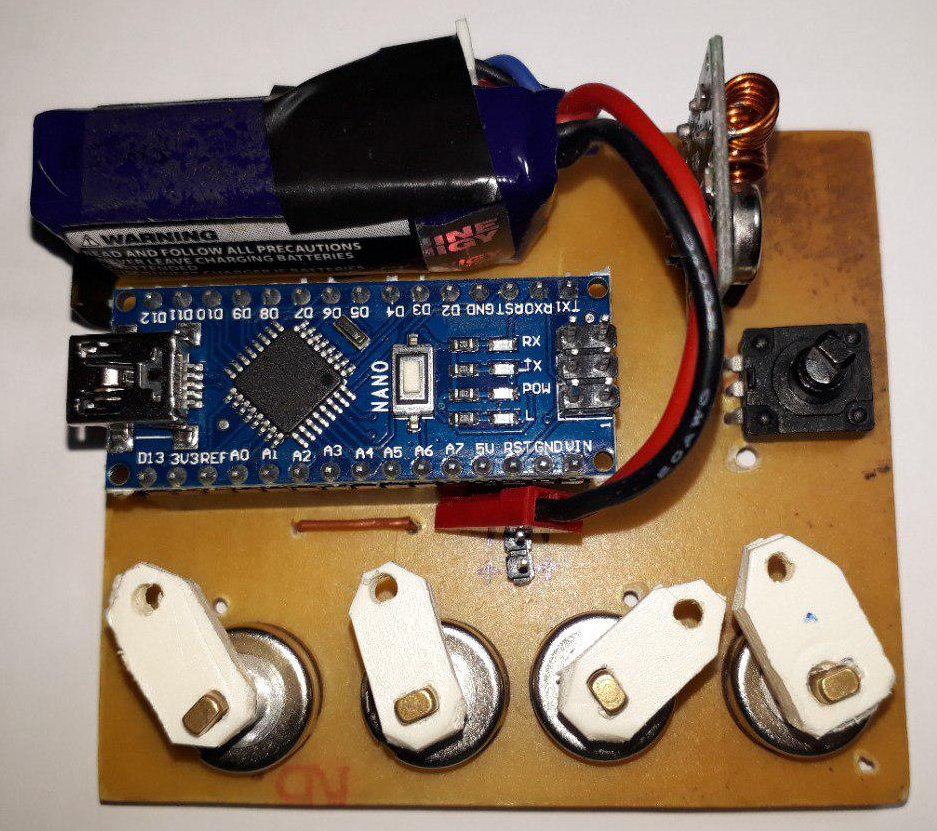
\includegraphics[width=7cm,keepaspectratio=true]{./figures/glove-module-ready1.jpg}
		 }
		 \label{Fig:phenolic-and-ready}
		 \fonte{Produzido pelo autor.}
	\end{figure}

%		\section{Montagem}

%		Utilizando uma luva de algodão, em seu dorso foi costurado uma das metades de um pedaço de velcro (gancho) de dimensões semelhantes à PCI contruída anteriormente. Ao longo dos dedos da luva foram costurados pequenos segmentos de plástico que serviriam como guias para os fios.	Na parte inferior da PCI foi costurada a outra metade do velcro (argola) que poderia ser fixada, sempre que fosse preciso, à outra parte do velcro costurada na luva.

%		Fios de náilon foram fixados nos segmentos de plástico (guias) localizados nas pontas dos dedos da luva. Os fios passavam por dentro das guias até serem amarrados em pequenos pedaços de PCV expandido que estavam conectados dos cursores dos potenciômetros. Por fim, pequenos pedaços de elástico, levemente esticados, também foram amarrados nos pedaços de PCV expandido.
		

		\begin{figure}[h!]
			\centering
			\caption{Luva montada.}
  		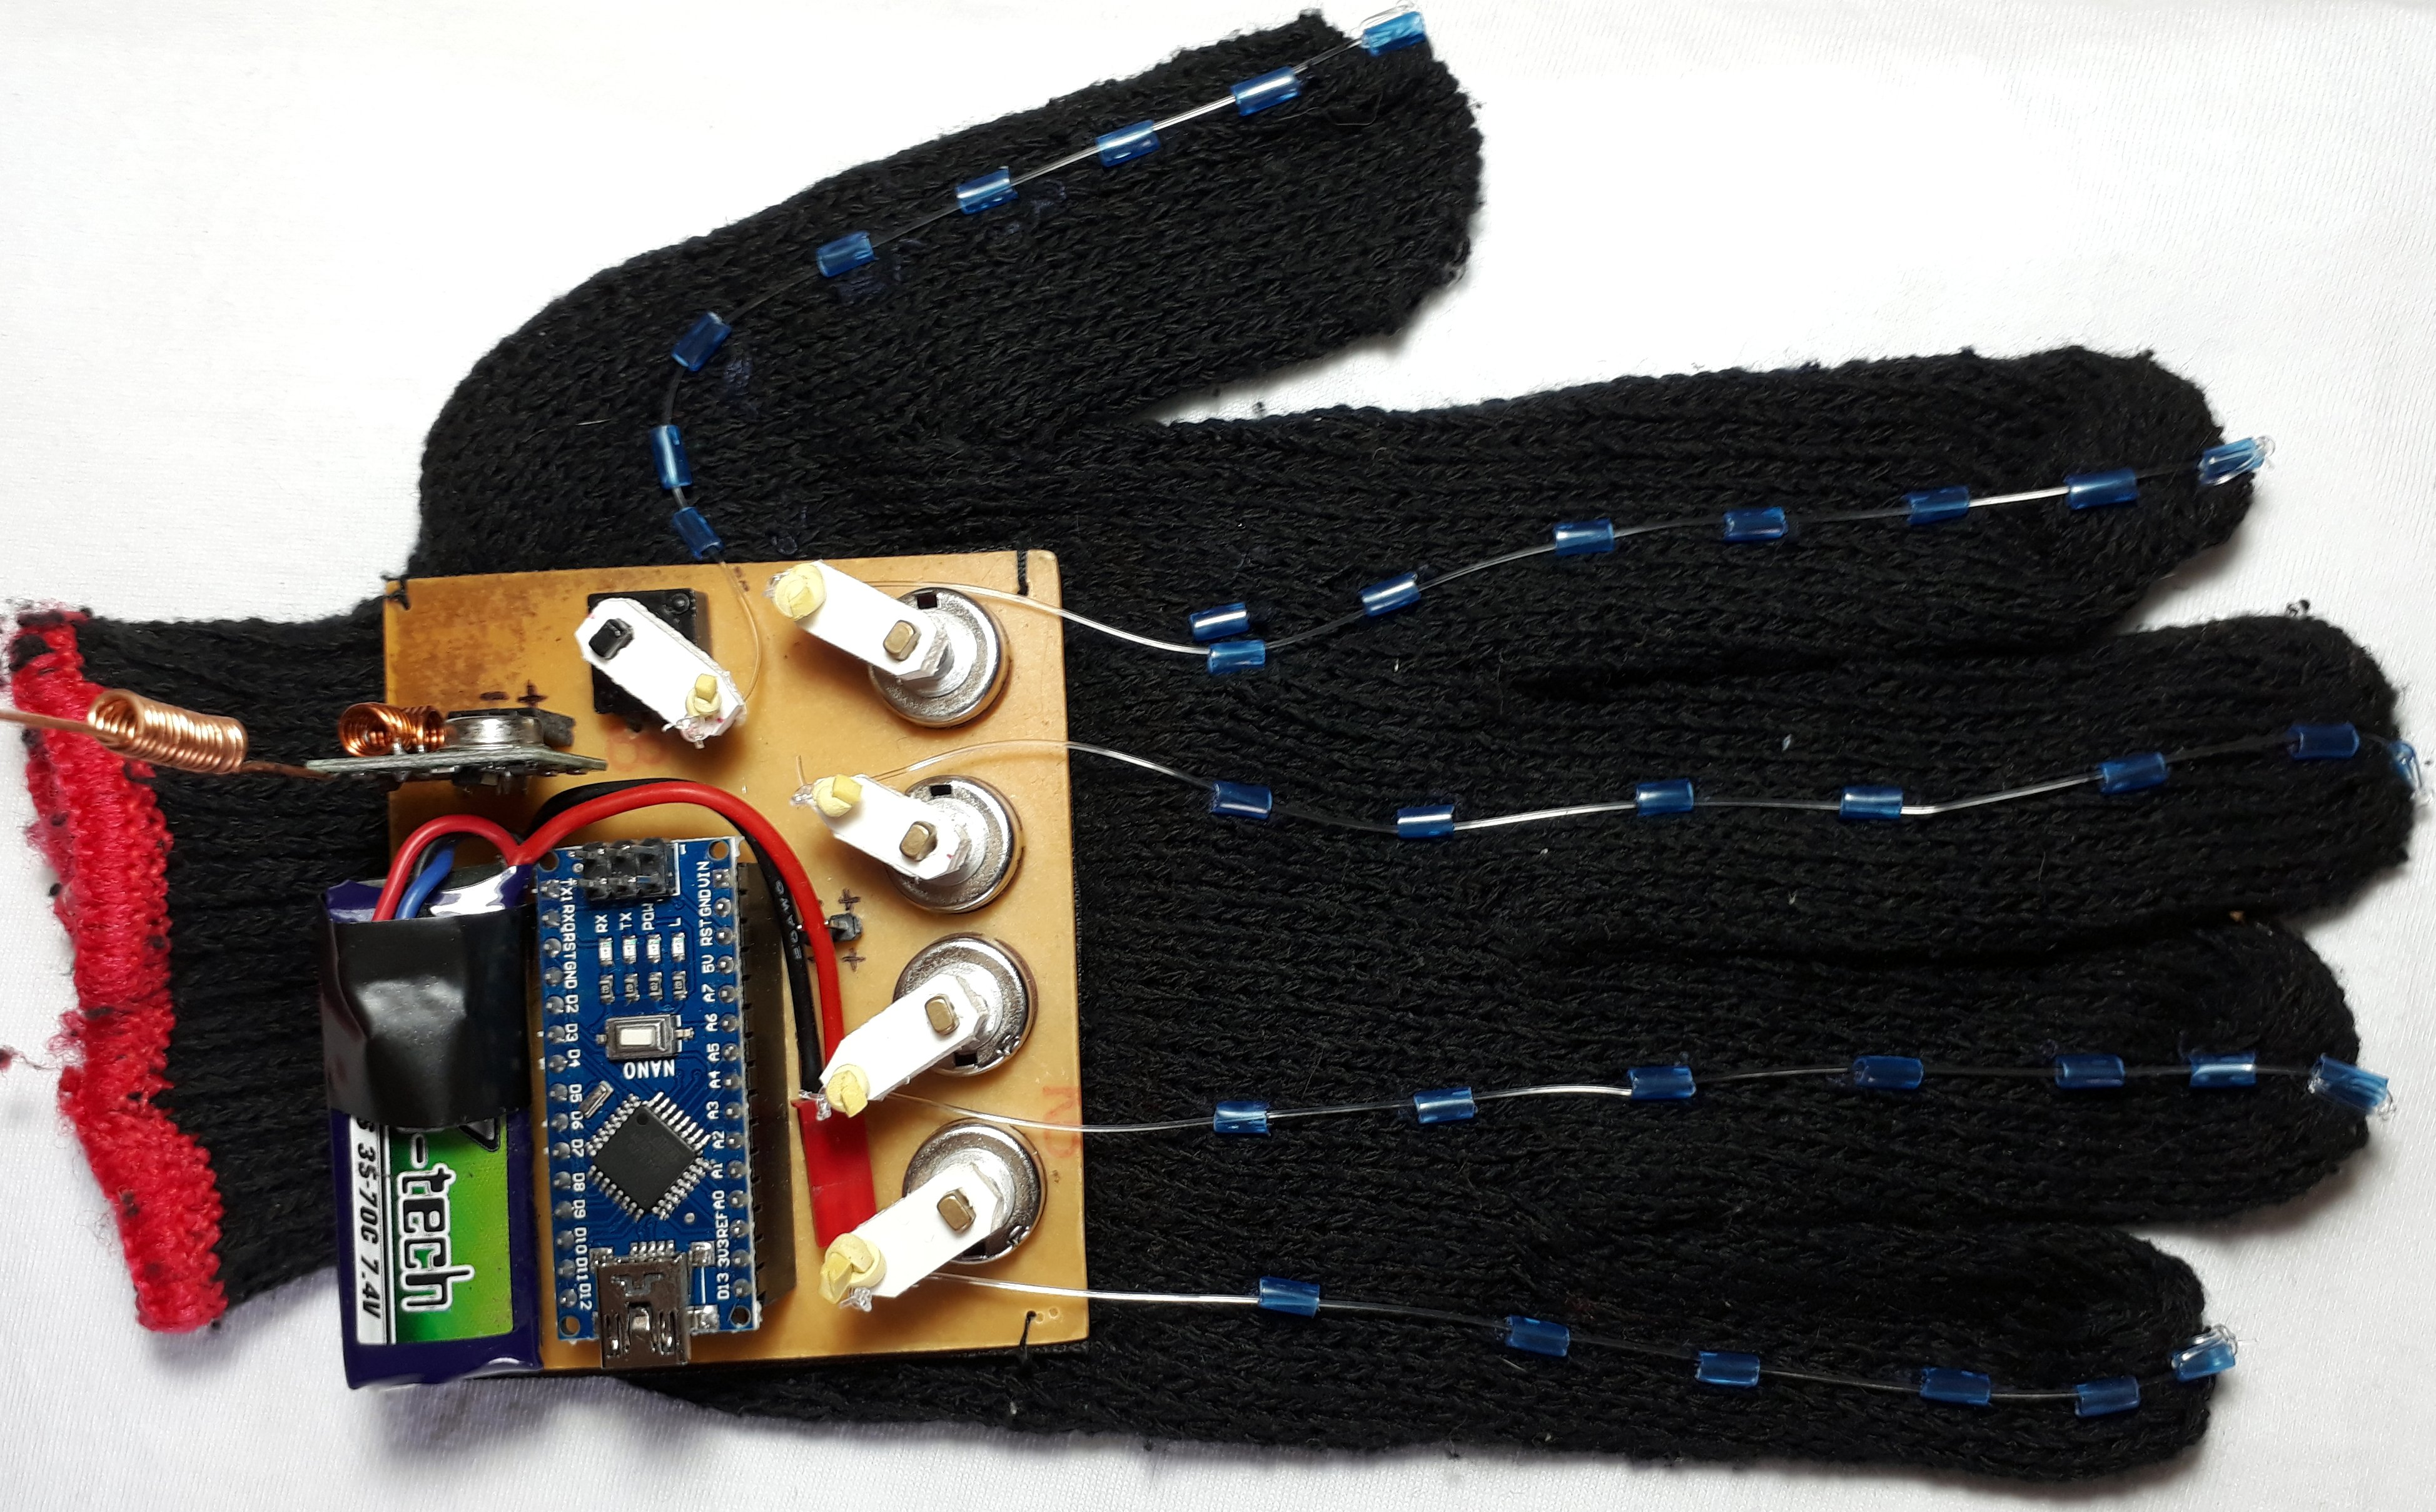
\includegraphics[width=14cm,keepaspectratio=true]{figures/glove-ready1.jpg}
  		\label{Fig:glove-ready1}
			\fonte{Produzido pelo autor.}
		\end{figure}




	% --------------------------------------------------
	%				RESULTADOS E ANÁLISES	
	% --------------------------------------------------




\chapter{Resultados e análises}

		\section{Introdução}

		O capítulo a seguir realiza diferentes testes com o sistema bioinspirado desenvolvido e os compara com outros trabalhos semelhantes. As três frentes a serem analisadas são: a sensibilidade do sensor de flexão, a duração do sistema alimentado por bateria e o alcance de transmissão do sinal.
		

		\section{Sensibilidade}

		O primeiro teste a ser realizado foi o teste de sensibilidade do sistema. Sendo este um sensor de flexão, faz-se necessário mensurar a quantidade máxima de posições capturadas em um movimento. Diversos trabalhos utilizam sensores flex comerciais para realizar a captura de movimentos. O desempenho de um desses trabalhos foi utilizado como referência.
%		\section{Sensor Flex}

		Os sensores de flexão comerciais, mais conhecidos como sensores flex, são resistores analógicos. Dentro desses sensores existem elementos resistivos de carbono junto a um fino substrato flexível. Quando o substrato é torcido o sensor produz uma resistência relativa ao raio da torção. Quanto maior o raio de torção maior será a resistência apresentada pelo sensor \cite{solanki2013sign}. A figura \ref{Fig:flex-sensor1} mostra um sensor flex da fabricante Spectra Symbol.

	\begin{figure}[!h]
		\centering
		\caption{Sensor de Flexão.}
		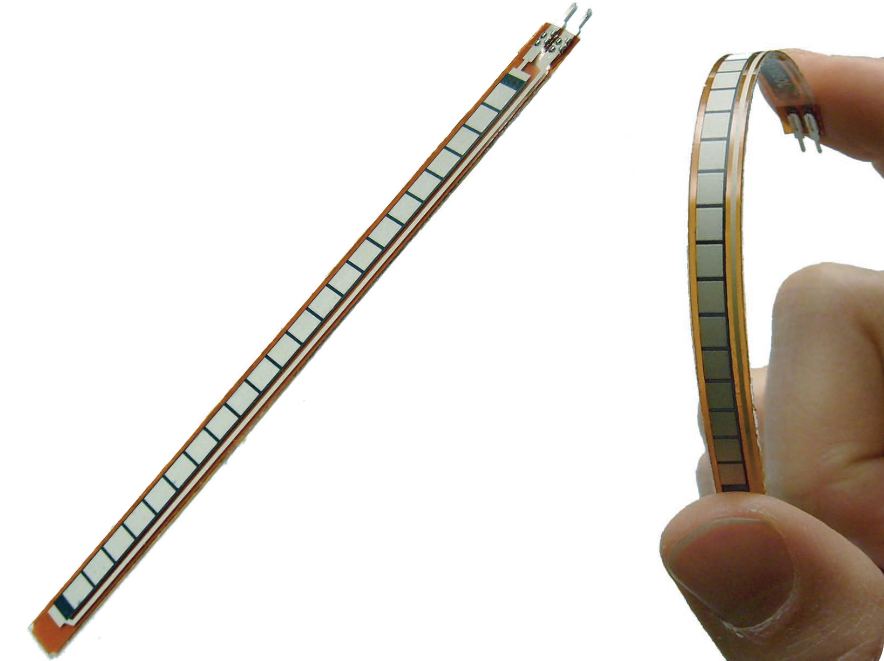
\includegraphics[width=7cm,keepaspectratio=true]{./figures/flex-sensor1.png}
		\fonte{\cite{flexsensor}.}
		\label{Fig:flex-sensor1}
	\end{figure}


		A figura \ref{Fig:hand-flexsensor-degrees1} demonstra uso do sensor flex comercial em um dos pontos de flexão do dedo. A figura também mostra o que seriam os graus de torção do sensor. À esquerda estão a mão e o sensor (em azul), em posição inicial, ambos com ângulo de flexão de aproximadamente 0 (zero) grau. À direita está o resultado de um movimento de flexão de aproximadamente 90 graus em relação à posição anterior.


	\begin{figure}[!h]
		\centering
		\caption{Sensor flex comercial na mão durante a flexão.}
		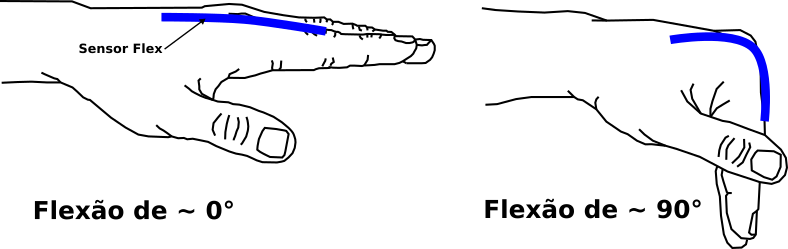
\includegraphics[width=13cm,keepaspectratio=true]{./figures/hand-flexsensor-degrees1.png}
		\fonte{Produzido pelo autor.}
		\label{Fig:hand-flexsensor-degrees1}
	\end{figure}

	
		O trabalho de \cite{anbarasi2013deafmute}, que será utilizado como referência, utiliza sensores flex comerciais de 2,5 e 4,5 polegadas instalados em uma luva, com o propósito de criar um interpretador da linguagem americana de sinais. Os gestos traduzidos são transformados em palavras que são exibidas em uma pequena tela de LCD.

		O autor cita que durante os testes, os sensores flex de 2,5 polegadas foram instalados nos dedos mínimo e polegar, enquanto que os sensores de 4,5 polegadas foram instalados nos dedos indicador, médio e anelar. Ele apresenta uma tabela de valores obtidos por cada sensor nas posições de flexão de 0 graus e 90 graus.

%		No sensor de flexão bioinspirado desenvolvido, para comparar com o trabalho de \cite{anbarasi2013deafmute}, com a luva vestida, foram obtidos os valores digitais captados nas duas posições da mão demostradas na figura \ref{Fig:hand-flexsensor-degrees1}.
		
		Os valores digitais obtidos nas posições de flexão de 0 grau e 90 graus, de ambos os trabalhos, foram utilizados para calcular, de acordo com as equações \ref{Eq:Desloca1} e \ref{Eq:NPos1}, o número de posições possíveis captadas entre 0 e 90 graus. Sendo que, para este cálculo, PosB recebe o valor digital em 90 graus e PosA recebe o valor digital recebido em 0 grau.

		A tabela \ref{Tab:NPos0-90} mostra os valores obtidos em 0 grau (Pos0), 90 graus (Pos90) e o número de posições possíveis (NPos) calculados. As duas colunas da esquerda são referentes ao sensor flex comercial e as demais são referentes aos dedos do sensor bioinspirado. O dedo polegar não está presente na tabela porque ele não é flexionado durante o movimento realizado neste teste.
		
		\begin{table}[H]
  	\centering
		\caption{Valores obtidos e número de posições entre 0 e 90 graus.}
    \begin{tabular}{l|ccccccc}
      \midrule
			Posições&\textcolor{red}{2,5''}	&\textcolor{red}{4,5''}	& Minimo	& Anelar	& Médio	&	Indicador	\\
      \midrule
			Pos0 		& 748 									& 350 									& 206 		&	142			&	771		&	746				\\
			Pos90 	& 875 									& 568 									& 309 		&	396			&	527		&	607				\\
			NPos 		& 128 									& 219 									& 104 		&	255			&	245		&	140				\\
      \midrule
    \end{tabular}
		\label{Tab:NPos0-90}
    \fonte{Adaptado de \cite{anbarasi2013deafmute} e produzido pelo autor.}
		\end{table}

		Através da tabela \ref{Tab:NPos0-90} é possível notar que o maior número de posições detectáveis neste teste é do dedo anelar do sensor bioinspirado, já o menor é do dedo mínimo. O sensor flex comercial de 4,5 polegadas apresenta desempenho superior aos dedos indicador e mínimo do sensor bioinspirado, já o modelo comercial de 2,5 polegadas, apresenta baixo desempenho, sendo superior apenas ao dedo mínimo.

		No desempenho geral, vemos que usando o sensor bioinspirado produzido, conseguimos captar um número superior de posições de flexão nos dedos anelar e médio, em comparação ao sensor flex de 4,5 polegadas. Em comparação com modelo de 2,5 polegadas, o sensor bioinspirado se sai melhor em 3 dos 4 dedos.

		Dessa forma é possível afirmar que, neste teste, o sensor bioinspirado conseguiu desempenho equiparado a um sensor comercial. Sendo que um sensor flex comercial possui um custo relativamente superior.




			\section{Bateria}

			A mobilidade é um dos requisitos do projeto desenvolvido. Por conta desse fato, a alimentação da luva é feita por uma pequena bateria LiPo. Outros projetos de luvas móveis também usam baterias ou até mesmo pilhas. O desempenho de cada projeto varia de acordo com o hardware implementado e a capacidade da fonte de alimentação. Nessa seção, o desempenho da bateria da luva produzida será comparado ao de outros projetos.

			A luva comercial Data Glove 5 Ultra da fabricante 5DT Inc. possui sensores de flexão baseados em fibra óptica. Esse produto pode ser utilizado para modelagem 3D e animação em programas de computador. Utiliza tecnologia de comunição sem fio Bluetooth e seu datasheet afirma um desempenho da bateria recarregável aproximado de 8 horas \cite{5DT-ultra}. Por ser um produto fechado, as características de sua bateria não são conhecidas.

			O trabalho de \cite{michela2013rehab} busca, através de uma luva sensorizada, mensurar a flexão dos dedos para estudos de reabilitação. A luva é embarcada com sensores flex comerciais, um microcontrolador e um transmissor de rádio frequência. Toda a eletrônica é alimentada por uma bateria em formato de botão com tensão nominal de 3$\,$V e capacidade de 1000$\,$mAh. Obteve desempenho aproximado de uma semana.
			
			Uma luva de baixo custo foi desenvolvida por \cite{simone2007lowcost} com o propósito de monitorar a flexão dos dedos de pessoas com disfunções na mão. A unidade possui sensores de flexão e uma placa embarcada com um microprocessador, uma memória RAM externa, um transmissor de sinal padrão IEEE 802.15.4 e pilhas AA alcalinas. A capacidade dessas pilhas não foi definida no trabalho, porém \cite{buchmann2016batteries} cita que esse tipo de pilha possui capacidade de até 2870$\,$mAh cada. Usando duas pilhas novas durante os testes, o sistema conseguiu ser alimentado por quase 60 horas.

			A luva bioinspirada desse trabalho está equipada com cinco potenciômetros, um microcontrolador Arduino, um transmissor de rádio frequência 433$\,$MHz e uma bateria LiPo com tensão nominal de 7,4$\,$V e capacidade de 300$\,$mAh. Essa bateria, apesar de possuir tensão nominal de 7,4$\,$V, consegue alcançar uma tensão de até 8,4$\,$V quando está totalmente carregada \cite{buchmann2016batteries}.

			É recomendado alimentar o Arduíno Nano com tensões entre 7$\,$V e 12$\,$V \cite{arduinopowerrange}, portanto, a luva funciona como esperado até o momento em que a tensão da bateria descarrega no limite de 7$\,$V. Em caso de uso contínuo a partir desse valor, o microcontrolador passa a reiniciar constantemente impossibilitando seu uso até que a bateria seja recarregada ou substituída.

			Para realizar o teste de desempenho da bateria, um módulo receptor junto a um Arduino foram conectados a um computador. Uma bateria recém carregada completamente, foi conectada à luva e o momento inicial foi marcado. O sistema transmissor da luva ficou ligado enviando sinais continuamente. Durante o teste, a tensão da bateria foi monitorada em intervalos regulares. Após um período de aproximadamente 10 horas a tensão da bateria chegou ao limite definido de 7$\,$V e o teste foi encerrado.

			A tabela \ref{Tab:battery-range} resume o desempenho dos dispositivos explicitados nesta seção.

%Característica de uso			
                          
%Modelagem 3D e animação 	
%Estudos de reabilitação 	
%Monitorar flexão dos dedos
%Controle de um carrinho		

		\begin{table}[H]
  	\centering
		\caption{Desempenho de alimentação das luvas}
    \begin{tabular}{c|c|c|c}
      \midrule
			Luva 								& Alimentação			&	Capacidade	& Duração	\\
      \midrule                                            					
			Data Glove 5				& Não definida		& Não definida& 8 horas \\
			Luva sensorizada 		& 1 bateria-botão	& 1000$\,$mAh		& 1 semana\\
			Luva de baixo custo & 2 pilhas AA			& 5740$\,$mAh		& 60 horas\\
			BioGlove						& 1 LiPo 7,4$\,$V			& 300$\,$mAh			&	10 horas\\	
      \midrule
    \end{tabular}
		\label{Tab:battery-range}
    \fonte{Produzido pelo autor.}
		\end{table}

		Analisando a tabela \ref{Tab:battery-range} percebe-se que a luva sensorizada possui o melhor desempenho, isso pode ser atribuído ao hardware de baixo consumo de energia e ao número reduzido de componentes do projeto \cite{michela2013rehab}. A luva de baixo custo desenvolvida em \cite{simone2007lowcost} também apresenta um desempenho excepcional, isto pode ser atribuído pela alta capacidade fornecida através de suas 2 pilhas alcalinas.

		A luva Data Glove 5, apesar de ser um produto comercial, possui o pior desempenho dentre todos os analisados, o hardware fechado dificulta a análise para além da duração de sua bateria. Porém, deve-se notar que esta luva apresenta diversos recursos de uso como calibração, compatibilidade com diversos sistemas operacionais e softwares \cite{5DT-ultra}. Portanto, seu consumo de energia elevado pode ser caracterizado pela provável complexidade do hardware deste produto.

		O segundo pior desempenho foi obtido pela BioGlove. Sua alimentação de baixa capacidade, o uso de uma placa comercial recheada de componentes e o envio constante de mensagens através de seu módulo transmissor podem ser as principais causas desse curto período de duração apresentado. Entretanto, pelo fato de a placa embarcada usar um Arduíno, este pode ser alimentado via cabo USB. Para aplicações que exigam um maior período de funcionamento ininterrupto, o uso do cabo USB poderia ser uma opção viável.

			\section{Alcance}

			Em um projeto móvel, o alcance do transmissor em relação ao receptor é limitado pela tecnologia empregada nesses equipamentos. Hardwares com maior potência alcançam maiores distâncias, entretanto tem custo mais elevado. Existem tecnologias de transmissão de baixo custo, como a que foi empregada nesse projeto, porém com alcance menor. 
			
			Dentre as diversas opções, há projetos que utilizam transmissão via bluetooth, que permite interação com computadores, smartphones ou qualquer outro dispositivo compatível que esteja próximo. Outros projetos chegam a usar a tecnologia de rede Wi-Fi e com isso são capazes de enviar comandos através da internet, podendo interagir com qualquer dispositivo conectado à grande rede mundial. 

			Na seção a seguir, o alcance de projetos de luvas que utilizam a tecnologia Bluetooth serão comparados ao método de transmissão via rádio frequência utilizado na luva bioinspirada produzida.

			O datasheet da luva comercial Data Glove 5 Utra ofecere também informações sobre sua tecnologia de transmissão. Nele está especificado que atrelado à luva há um kit de transmissão sem fio, no qual suporta até duas luvas simultaneamente. A tecnologia de transmissão Bluetooth utilizada, trabalha na faixa de 2,4$\,$GHz e consegue um alcance de até 20 metros \cite{5DT-ultra}.

			PERCRO Dataglove é uma luva baseada no funcionamento de goniômetros, que são instrumentos responsáveis por medir o deslocamento angular relativo. Desenvolvida no trabalho de \cite{rodriguez2007goniometric}, possui dois sensores em cada dedo, um microcontrolador embarcado e um módulo Bluetooth 2,4$\,$GHz que chega a alcançar uma comunicação satisfatória de até 10 metros.

			A BioGlove está equipada com um par de módulos de transmissão e recepção de rádio frequência que trabalham na faixa de 433$\,$MHz. De acordo com o manual da biblioteca que auxilia o uso desse equipamento, usando uma antena de 17$\,$cm em ambos os módulos, o alcance pode ser de até 150 metros em campo aberto \cite{virtualwiremanual}. Entretanto, por conta da fragilidade dos módulos, foi possível soldar apenas uma antena no transmissor.

			Durante os testes de alcance de transmissão, o módulo receptor foi conectado a um computador que ficou fixo em um local. O transmissor embarcado na luva foi sendo distanciado aos poucos enquanto que a resposta do receptor era constantemente verificada. Por volta de 7,5 metros a resposta do transmissor começou a falhar e o teste foi encerrado nesta marca. A tabela \ref{Tab:wifi-range} resume o desempenho de alcance apresentado pelas três luvas.

		\begin{table}[H]
  	\centering
		\caption{Desempenho de alcance das luvas}
    \begin{tabular}{c|c|c|c}
      \midrule
			Luva 						& Tecnologia			&	Faixa		& Alcance		\\
      \midrule                                            					
			Data Glove 5		& Bluetooth				& 2,4$\,$GHz	& 20 metros	\\
			PERCRO Dataglove& Bluetooth				& 2,4$\,$GHz	& 10 metros	\\
			BioGlove				& Rádio Frequência& 433$\,$MHz	&	7,5 metros\\	
      \midrule
    \end{tabular}
		\label{Tab:wifi-range}
    \fonte{Produzido pelo autor.}
		\end{table}

			Observa-se pela tabela \ref{Tab:wifi-range} que apesar de duas luvas usarem a mesma tecnologia, apresentam resultados diferentes. Isso pode ser atribuído à diferentes versões dos módulos ou à potência empregada neles. A luva comercial mostrou possuir o melhor desempenho chegando a ter o dobro do alcance útil em relação à segunda colocada.

			O pior desepenho ficou por conta da BioGlove, esta que emprega uma tecnologia de comunicação mais barata, apresentando desempenho muito inferior ao indicado no manual. Apesar disso, conseguiu um alcance relativamente próximo ao da PERCRO Dataglove. Além disso, deve ser lembrado que o módulo receptor da BioGlove não recebeu uma antena, o que poderia potencializar o alcance de comunicação do par.




	% ----------------------------------------
	%							CONCLUSÃO	
	% ----------------------------------------



		\chapter{Conclusão}

		Este trabalho se mostrou viável em comparação à outras soluções semelhantes, mesmo frente à um produto comercial. Em 2 dos 3 aspectos pesquisados, a BioGlove conseguiu se equiparar à outros projetos. O principal ponto de pesquisa da luva, o sensoriamento de flexão, em alguns momentos chegou até mesmo a ser superior ao sensor flex comercial amplamente utilizado em diversos projetos.

		Sua bateria de baixa capacidade apresentou um desempenho relativamente curto durante o uso ininterrupto, porém, quando comparado à um produto comercial completo, conseguiu durar ligeiramente por mais tempo. O alcance de transmissão da BioGlove foi o aspecto com pior desempenho, frente à tecnologia Bluetooth utilizada em outras luvas. 

		Após a análise dos resultados que se apresentaram menos animadores, é possível perceber que pequenas mudanças podem influenciar na melhoria do desempenho em futuros testes. A vida útil da luva pode ser melhorado pelo uso de uma bateria mais potente e pelo aperfeiçoamento da frequência da transmissão de mensagens, enviar apenas quando for necessário, e não a todo momento como acontece atualmente. A inclusão de antenas melhores em ambos os módulos de rádio frequencia ou a troca da tecnologia de transmissão, por Bluetooth por exemplo, pode garantir uma melhoria no alcance de transmissão.

		Os maiores desafios se apresentaram durante a escolha de componentes e montagem da luva. Não havendo muitas referências de trabalhos com mecânica semelhante, durante a montagem, os problemas inesperados foram sendo resolvidos com uso de componentes e ferramentas disponíveis no momento, mesmo que esses não fossem os ideais. Portanto, a troca de componentes por outros mais precisos, menores e que consumam menos energia, podem garantir maior estabilidade à luva.

		O protocolo de comunicação criado, mesmo sendo simples, conseguiu chegar satisfatoriamente ao seu objetivo inicial de controlar os movimentos do carrinho, tendo a possibilidade até mesmo ser aproveitado para outras aplicações de controle. Entretanto, para aplicações que exijam uma demanda maior transmissão de dados, e não apenas 5 \textit{bytes} por mensagem, será necessária uma melhoria no protocolo ou até mesmo a substituição do mesmo.

		Este protótipo foi desenvolvido, usado e testado por apenas uma pessoa, o uso da luva por outras pessoas pode apresentar resultados diferentes e necessitar de ajustes. Cada pessoa possui características diferentes em suas mãos, dedos maiores ou menores, mão mais larga ou mais fina, diferentes graus de flexão dos dedos, entre outros. Portanto, a inclusão de uma função de calibração no software é necessária e pode diminuir tais contratempos quando a BioGlove for utilizada por outros indivíduos.

		Apesar de no geral o projeto desenvolvido se mostrar viável para ser uma luva de aferição de movimentos e transmissão de dados, este possui natureza diferente de outros produtos semelhantes. Enquanto que o uso de sensores flex pode trazer uma mecânica relativamente estável durante os movimentos, a BioGlove é dependente de uma rede de fios e polias que não apresentou muita estabilidade mecânica em uma luva de algodão. A troca do material da luva por um  mais rígido, poderia favorecer a estabilidade durante os movimentos.

		Com tudo, a BioGlove, mesmo apresentando limitações, se mostra capaz de fomentar projetos de baixo custo que necessitem desse tipo de equipamento. O uso de componentes de baixo custo, como potenciômetros e o par RF, além da amplamente conhecida e documentada placa Arduíno, permite com os devidos ajustes, que diversos módulos compatíveis sejam adicionados ao projeto. Com isso há a possibilidade de desenvolver soluções mais complexas, como a tradução da Linguagem Brasileira de Sinais (LIBRAS) de gestos para palavras ou até mesmo a interação com softwares de realidade virtual.

			\section{Trabalhos futuros}		

		Dentre os possíveis trabalhos futuros relacionados à esse projeto estão:

		\begin{itemize}
			\item Investigar o uso de uma luva composta de material mais resistente do que o algodão.
			\item Usar um número maior de polias para guiar o fio utilizado.
			\item Investigar o uso de módulos com outras tecnologias de transmissão de dados.
			\item Trocar a bateria por outra de maior capacidade.
			\item Usar potênciometros de menor tamanho e menor resistência elétrica.
			\item Substituir a placa Arduíno pelo uso apenas do microcontrolador ATmega.
			\item Criar uma função de calibração para uso da luva.
			\item Aumentar o número de \textit{bytes} na mensagem transmitida.
			\item Modificar o software para enviar dados apenas quando for necessário.
			\item Diminuir o tamanho da PCI embarcada na luva.
		\end{itemize}









%		\chapter{BUFFER}
%		Também é possível notar que alguns deslocamentos são positivos enquanto outros são negativos. Isso se dá porque os potênciometros 1 e 2 foram instalados com seus cursores em sentido oposto aos potenciômetros 3 e 4. Com o intuito de minimizar o espaço entre eles na placa. Isso pode ser observado na figura \ref{Fig:glove-ready1}.
%
%		Por conta desse fato, durante o movimento de flexão, os potenciômetros 1 e 2 giram em sentido anti-horário e possuem deslocamento positivo, enquanto os demais giram em sentido horário com deslocamento negativo. No caso do potenciômetro 5, apesar de girar em sentido anti-horário, ele possui um deslocamento negativo. Isso porque foi soldado em posição reversa aos demais, com o propósito de maximar sua aderência na placa.
%
%		\section{Transmissão e Recepção de Dados}
%
%			Como foi descrito, durante a movimentação dos dedos, a posição do cursor do potenciômetro é modificado. Sendo assim, para possibilitar o sensoriamento, a variação de cada potenciômetro é captada por um microcontrolador que processa esse sinal antes de despachá-lo para o transmissor. Este por sua vez envia mensagens por rádio frequência, em formato de números inteiros que representam a posição atual de cada dedo. Figura \ref{Fig:transmitter-and-receptor} (a).
%
%			O módulo receptor de rádio frequência, capta as mensagens e as envia a outro microcontrolador. Este por sua vez, processa a mensagem e transmite aos respectivos componentes e atuadores daquela aplicação. Figura \ref{Fig:transmitter-and-receptor} (b).
%
%	\begin{figure}[!htb]
%  	\centering
%   	\caption{ (a) Transmissão do sinal. (b) Recepção do sinal.}
%   	\subfloat[]
%  	{
%     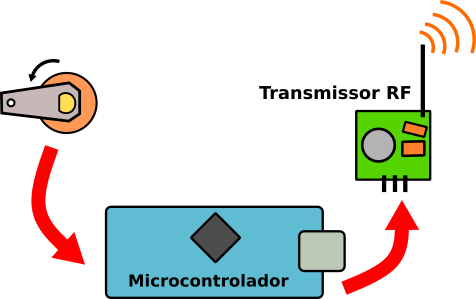
\includegraphics[width=7cm,keepaspectratio=true]{./figures/transmitter-module1.png}
%    }
%   	\centering
%   	\subfloat[]
%   	{ 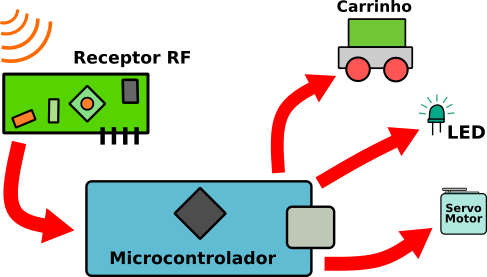
\includegraphics[width=7cm,keepaspectratio=true]{./figures/receptor-module1.png}
%   	}
%  	\label{Fig:transmitter-and-receptor}
%   	\fonte{Produzido pelo autor.}
% 		\end{figure}
%
%			Para este trabalho, um pequeno carrinho, foi o sistema escolhido para ser controlado pela luva. Para isso, um protocolo de transmissão foi desenvolvido para traduzir os movimentos dos dedos da luva em direções para o carrinho.
%

	
		
% ----------------------------------------------------------
% ELEMENTOS PÓS-TEXTUAIS
% ----------------------------------------------------------
\postextual
% ----------------------------------------------------------
% Referências bibliográficas
% ----------------------------------------------------------
\bibliography{referencias}

%---------------------------------------------------------------------
% INDICE REMISSIVO
%---------------------------------------------------------------------

\printindex

\end{document}
